\documentclass{article}

\usepackage[utf8]{inputenc}
\usepackage{amssymb}
\usepackage{amsmath}
\usepackage{mathabx}
\usepackage{dcolumn}
\usepackage{geometry}
\usepackage{breqn}
\usepackage{graphicx}
\usepackage{float}
\usepackage{mathrsfs}
\usepackage{array}
\usepackage{caption}
\usepackage{subcaption}
\usepackage[spanish,es-lcroman]{babel}
\usepackage{enumerate}
\usepackage{nicefrac} 
\usepackage[most]{tcolorbox}
\usepackage{tcolorbox} % For solution boxes
%\decimalpointf
\setlength\parindent{0pt}
\usepackage{enumitem}
\newcommand*{\QED}{\hfill\ensuremath{\blacksquare}}
%\usepackage{authblk}
\selectlanguage{spanish}
\geometry{letterpaper, margin=1in}
\pagestyle{headings}
\usepackage{amsthm} 
\newtheorem{theorem}{Teorema}[section]
\newtheorem{corollary}{Corolario}[theorem]
\newtheorem{lemma}[theorem]{Lema}
\theoremstyle{remark}
\newtheorem*{remark}{Considere}
\DeclareUnicodeCharacter{2212}{-}
\usepackage{epigraph}
\usepackage{booktabs}
\usepackage{xcolor}
\usepackage[colorlinks = true]{hyperref}
\usepackage[backend=biber, style=apa]{biblatex}
\addbibresource{ref.bib}

%\usepackage[natbibapa]{apacite}
\usepackage{tikz}

\tcbset{colback=blue!10, 
    %colframe=green!45!black!20, 
    colframe=blue!70!black!70, 
    title=Soluci\'on,
    fonttitle=\bfseries,  
    coltitle=white,
    standard jigsaw, opacityback=50, arc=0mm, breakable} 

\newcommand{\ubar}[1]{\text{\b{$#1$}}}
 
\theoremstyle{definition}
\newtheorem{definition}{Definici\'on}[section]

\title{\textbf{Tendencia, Estacionalidad, Ciclos y Volatilidad} \\ {\Large Series de Tiempo para Pron\'osticos en Econom\'ia y Finanzas} \\ {\large Taller 2}}
\author{Nicolas Lozano Huertas\thanks{\href{mailto:n.lozanoh@uniandes.edu.co?subject= Taller 2 Series de Tiempo}{Universidad de los Andes}} \and Juan José Gutierrez \and Sof\'ia Prada \and Valentina Rond\'on}
\date{Abril, 2025}

\begin{document}

\maketitle
\vspace{-1 cm}
\section{[10 puntos] Modelos ARCH.}
{Lea el ``Nobel Lecture'' de Robert Engle para m\'as informaci\'on de los modelos ARCH.}
\begin{enumerate}[label = \emph{\alph*})]
    \item {Hagan un resumen de no m\'as de una p\'agina sobre esta lectura.}
        \begin{tcolorbox}[title=Soluci\'on 1.a]
            En su Nobel Lecture, \cite{engle2004}, busca exponer las principales car\'acteristicas de los modelos GARCH, su historia y algunas aplicaciones en mercados financieros. \\
            El autor comienza haciendo una breve introducci\'on en la cual resalta la importancia de medir y conocer el riesgo donde resalta que hay riesgos que se asumen porque los beneficios esperados superan los costos. Esta lógica es central en finanzas y dio origen a modelos como los de Markowitz, Tobin, Sharpe y Black-Scholes, que buscaron cuantificar y gestionar el riesgo, inicialmente a través de la varianza y posteriormente, a través de la volatilidad. 
            
            Para medir la varianza de forma más realista, Engle propuso el modelo ARCH que estima la varianza condicional con base en errores pasados otorgando mayor peso a la información reciente. Esto permitió capturar la naturaleza dinámica de la volatilidad. Por otra parte, Bollerslev amplió este enfoque con el modelo GARCH, que incorpora memoria en la serie y explica cómo la volatilidad responde a nueva información. Posteriormente, Nelson introdujo el modelo EGARCH, que permitió considerar respuestas asimétricas, las caídas en los precios aumentan más la volatilidad que las subidas. 
            
            El éxito de estos modelos permitió que se volvieran fundamentales en el análisis financiero ya que los rendimientos analizados presentan características comunes como imprevisibilidad, colas pesadas y agrupamiento de volatilidad. Por lo tanto, modelos como el GARCH(1,1) en particular, ha demostrado ser útil para describir estas dinámicas en activos de todo tipo reflejando cómo la llegada de nueva información afecta la volatilidad de los mercados financieros. Además de estimar el modelo, es necesario explicar las causas y los efectos de la volatilidad en la economía así que se menciona que en los mercados financieros las consecuencias de la volatilidad son fáciles de describir aunque difíciles de medir. Específicamente, se argumenta que un aumento en la volatilidad debería llevar a los inversores a vender ciertos activos, lo que provoca una caída en los precios para equilibrar el mercado. Este nuevo precio más bajo, a su vez, aumenta el rendimiento esperado en compensación por el riesgo adicional. Posterior a esta explicación en el texto, se realiza un análisis extenso del índice Standard and Poor's 500 (S\&P 500) desde 1963 hasta finales de noviembre de 2003 como ejemplo. Para ello, se realizan pronósticos de volatilidad utilizando modelos ARCH/GARCH y estimando los parámetros del modelo a través del método de Máxima Verosimilitud. Los resultados confirman que se observa que existen patrones empíricos de volatilidad en el S\&P 500 que reflejan dinámicas complejas y cambios significativos a lo largo del tiempo como lo fue la crisis financiera de 2008 o la pandemia de COVID-19. Además, que la volatilidad observada no es constante y que las predicciones de volatilidad afectadas por sus expectativas a cambios en factores fundamentales, como tasas de interés, políticas monetarias, y condiciones macroeconómicas pueden ser utilizadas para informar decisiones de inversión y gestión de cartera. 
            Por otra parte, el autor expone el Valor en Riesgo (VaR), el cual es utilizado por instituciones financieras para proporcionar información limitada sobre las probabilidades de pérdida que podrían ocurrir en la cartera donde cada día. El cálculo del VaR requiere supuestos sobre la distribución de los retornos y el comportamiento de la volatilidad. Aunque muchas veces se asume normalidad y volatilidad constante, los modelos dinámicos como TARCH permiten capturar mejor la realidad del mercado, considerando variaciones en la volatilidad y asimetrías en los retornos. A su vez, el texto analiza la práctica financiera de valorar opciones, enfocándose en la insuficiencia de los métodos tradicionales de valoración libre de arbitraje, como Black-Scholes, para capturar adecuadamente el riesgo y determinar precios justos en escenarios reales. Se propone complementar este enfoque con modelos fundamentales que incluyan costos de transacción, cobertura y riesgos de portafolio. A través de una simulación con modelos ARCH asimétricos (como el TARCH), se ilustra cómo calcular el valor de opciones put sobre el S\&P 500 con 10 días hasta el vencimiento. Los resultados muestran precios de opciones con formas esperadas (monótonamente crecientes y convexas), pero diferentes a los de Black-Scholes, reflejando volatilidades implícitas variables según el precio de ejercicio, fenómeno conocido como "sesgo de volatilidad". Este sesgo, confirma la utilidad de los modelos de volatilidad asimétrica. Sin embargo, también sugiere que los inversionistas valoran especialmente la protección contra grandes pérdidas, lo que exige una mejor aproximación a la neutralización del riesgo en las simulaciones, como han señalado diversos estudios. 

            Finalmente, el texto enfatiza en que la investigación futura se enfocará en desarrollar y aplicar modelos que utilicen mejor los datos de alta frecuencia y que gestionen la complejidad de las interacciones entre múltiples activos en el contexto financiero. 
        \end{tcolorbox}
    \item {¿De acuerdo a la lectura, cu\'ales son las caracter\'isticas de los datos financieros y macroecon\'omicos que los modelos ARCH pueden capturar?}
        \begin{tcolorbox}[title=Soluci\'on 1.b]
            
        \end{tcolorbox}
\end{enumerate}

\section{[45 puntos] Pron\'ostico de Variables Financieras.}

{En el archivo de Excel que se llama ``TRM'' que se encuentra en la carpeta de este taller, se tienen los datos de la tasa representativa de mercado diaria del peso colombiano con respecto al d\'olar de Estados Unidos, desde el 1 de diciembre del año 1991 hasta el 25 de marzo del año 2025.}

\begin{enumerate}[label = \emph{\alph*})]
    \item {Construya una serie mensual hist\'orica con la TRM promedio mensual desde diciembre del año 1991 hasta marzo del año 2025. Grafiquen la serie hist\'orica de la TRM construida y analicen los hechos m\'as relevantes que han generado variaciones en la TRM en el presente siglo. No es necesario un an\'alisis exhaustivo, s\'olo los principales hechos asociados a cambios fuertes en la serie observada.}
        \begin{tcolorbox}[title=Soluci\'on 2.a]
            \begin{figure}[H]
                \centering
                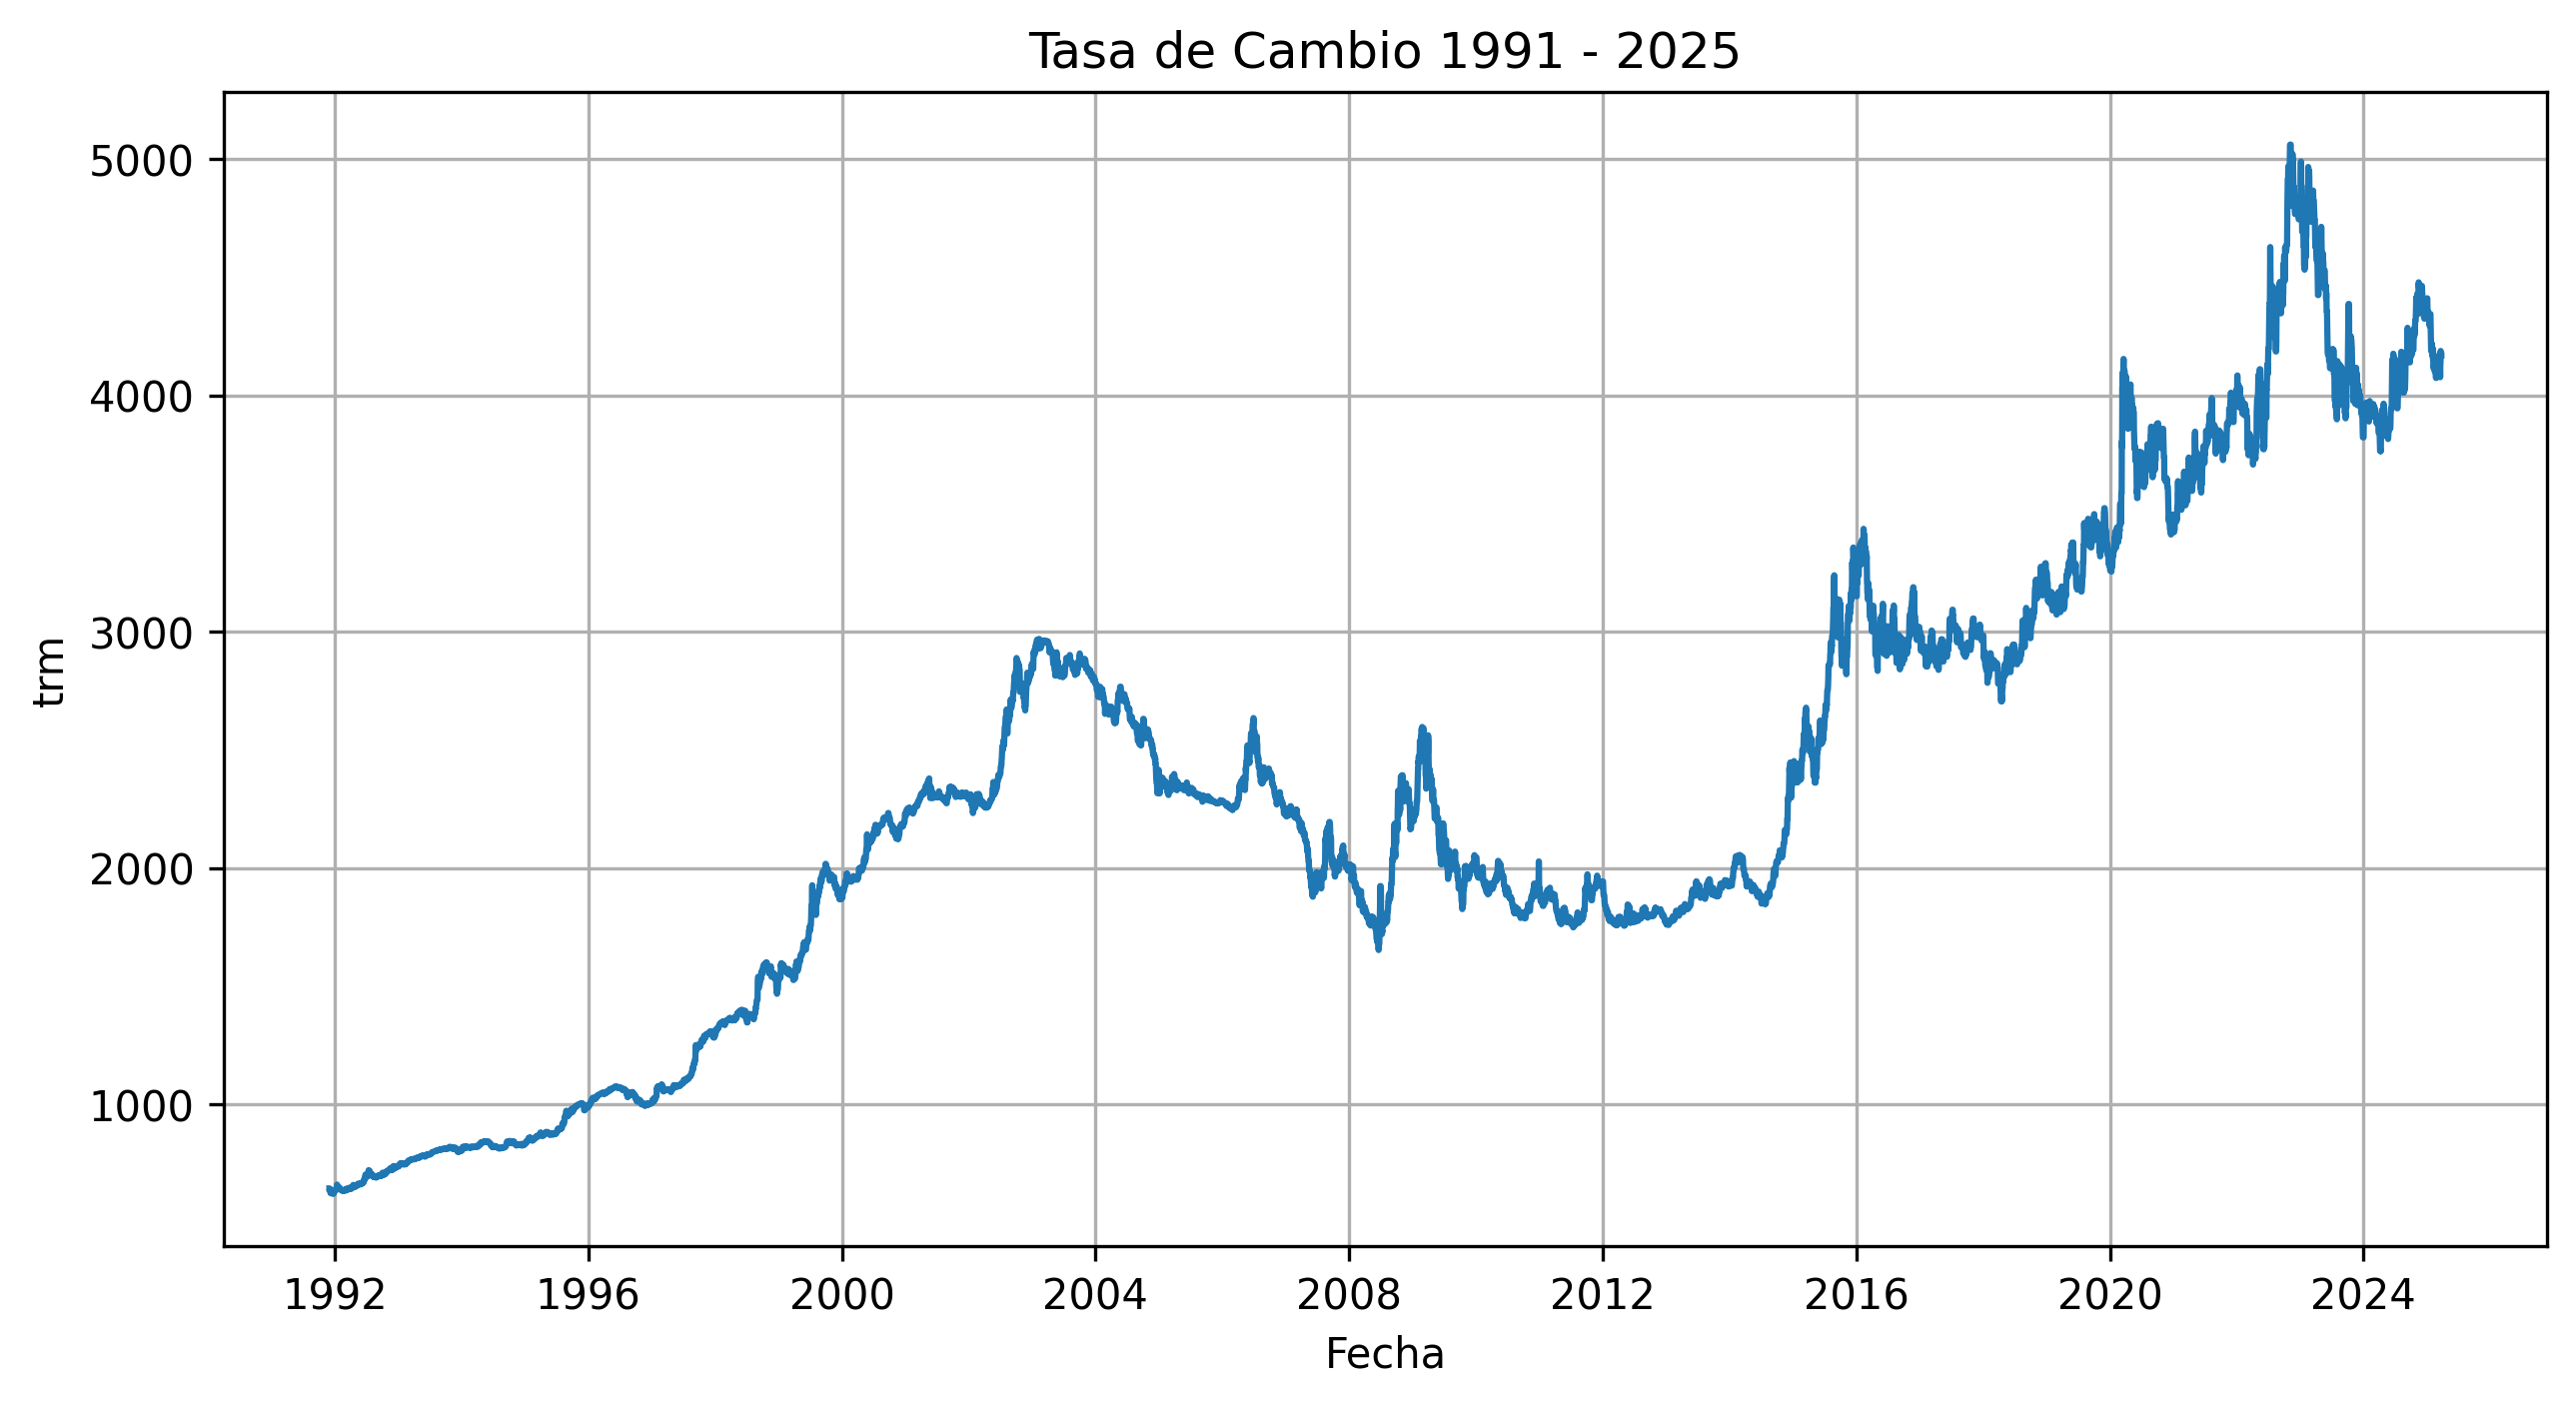
\includegraphics[width=0.9\linewidth]{output/graf_trm.png}\
                \caption{Serie TRM}
                \label{fig:serie_trm}
            \end{figure}

En la gráfica anterior podemos observar la evolución del promedio mensual de la tasa de cambio entre 1991 y 2025. En esta, los principales cambios que esta presenta son:
\begin{itemize}
    \item En el año 2004, la TRM presento un gran cambio en la tendencia que presentaba previamente. Específicamente, se presencia una caída continua en la TRM desde este año, frente a la tendencia creciente que presentaba antes. Este cambio se debe probablemente al déficit fiscal y comercial que llevaba Estados Unidos desde varios años atrás (\href{https://www.eltiempo.com/archivo/documento/MAM-1644518}{Gaviria, 2005}). 
    \item En el año 2008, la TRM presentó un agudo aumento, muy seguramente debido al inicio de la crisis financiera del 2008. Esta crisis generó altos niveles de volatilidad (nunca antes vistos) en la TRM (\href{https://www.portafolio.co/economia/finanzas/volatilidad-dolar-2008-alta-historia-debido-crisis-financiera-226460}{Portafolio, 2005}). 
    \item En el año 2014-2015, la TRM pasa de mantenerse estable a tener un considerable aumento, hasta el 2016. Este aumento inicial coincidió con la caída de los precios del petróleo (\href{https://www.banrep.gov.co/es/recuadro-1-perturbaciones-tasa-cambio-e-inflacion-colombia}{Banco de la República, 2016}), que ocurrió por un exceso de oferta y la decisión de la OPEP de continuar la producción.
    \item En el 2022, la TRM presenta una pico y subsecuente caída, que se explica en parte por las políticas aplicadas por la Reserva Federal, la buena calificación de la economía colombiana por organizaciones como el Fondo Monetario Internacional, y un cambio de postura frente al gobierno de Gustavo Petro (\href{https://www.udea.edu.co/wps/portal/udea/web/inicio/udea-noticias/udea-noticia/!ut/p/z0/fY69DsIwDIRfhaUjcighwFgxICEGBoRaL8i0FRjSuD8B8fgkMCAWFsvf-e5kQMgBHT34TJ7FkQ1coDkulqt0kmm1VUYblZmdns3T9XR_ULAB_G8IDXztOswAS3G-fnrIW-k92XtVU6Jo-KWLNPVnj3PkxHPJNCTqnXZcSXR9ZWnZhV_j3UpzYhpXYqmH9obFCxRvs5U!}{Valencia, 2023}). 
\end{itemize}


        \end{tcolorbox}
    \item {Estimen el retorno mensual de la TRM:}
    \begin{equation}
        r_t = (\ln(TRM_t) - \ln(TRM_{t-1})) \times 100
    \end{equation}
    {donde TRM$_t$ es la TRM promedio en el mes $t$. Calcule el valor promedio de dicha serie y rep\'ortelo. ¿En promedio los retornos de la TRM son positivos, negativos o cero?}
        \begin{tcolorbox}[title=Soluci\'on 2.b]
        
            \begin{table}[H]
\caption{Retorno Promedio}
\label{tab:retorno_promedio}
\begin{tabular}{lr}
\toprule
Estad\'istico & Valor \\
\midrule
Retorno Promedio & 0.015357 \\
\bottomrule
\end{tabular}
\end{table}


El promedio del retorno mensual de la TRM entre 1991 y 2025 es de 0.47\%, valor que, aunque es positivo, es muy valor muy pequeño. 
        \end{tcolorbox}
    \item {Estime el retorno mensual sin media y eleve dicha medida al cuadrado de la siguiente manera: }

    \begin{equation}
        r_t^2=[r_t-\bar{r}]^2
    \end{equation}

    {Donde $r_t$ es el valor de los retornos mensuales y $\bar{r}$ es el valor promedio de los retornos mensuales.} \\
    
    {Presente en dos gr\'aficas (tipo subplot) los retornos mensuales $r_t$ de la TRM y los retornos al cuadrado. Describa las gr\'aficas e interprete sus resultados a la luz de los an\'alisis realizados en clase y a partir de lo analizado en los hechos hist\'oricos descritos en el segundo apartado.}
        \begin{tcolorbox}[title=Soluci\'on 2.c]
            \begin{figure}[H]
                \centering
                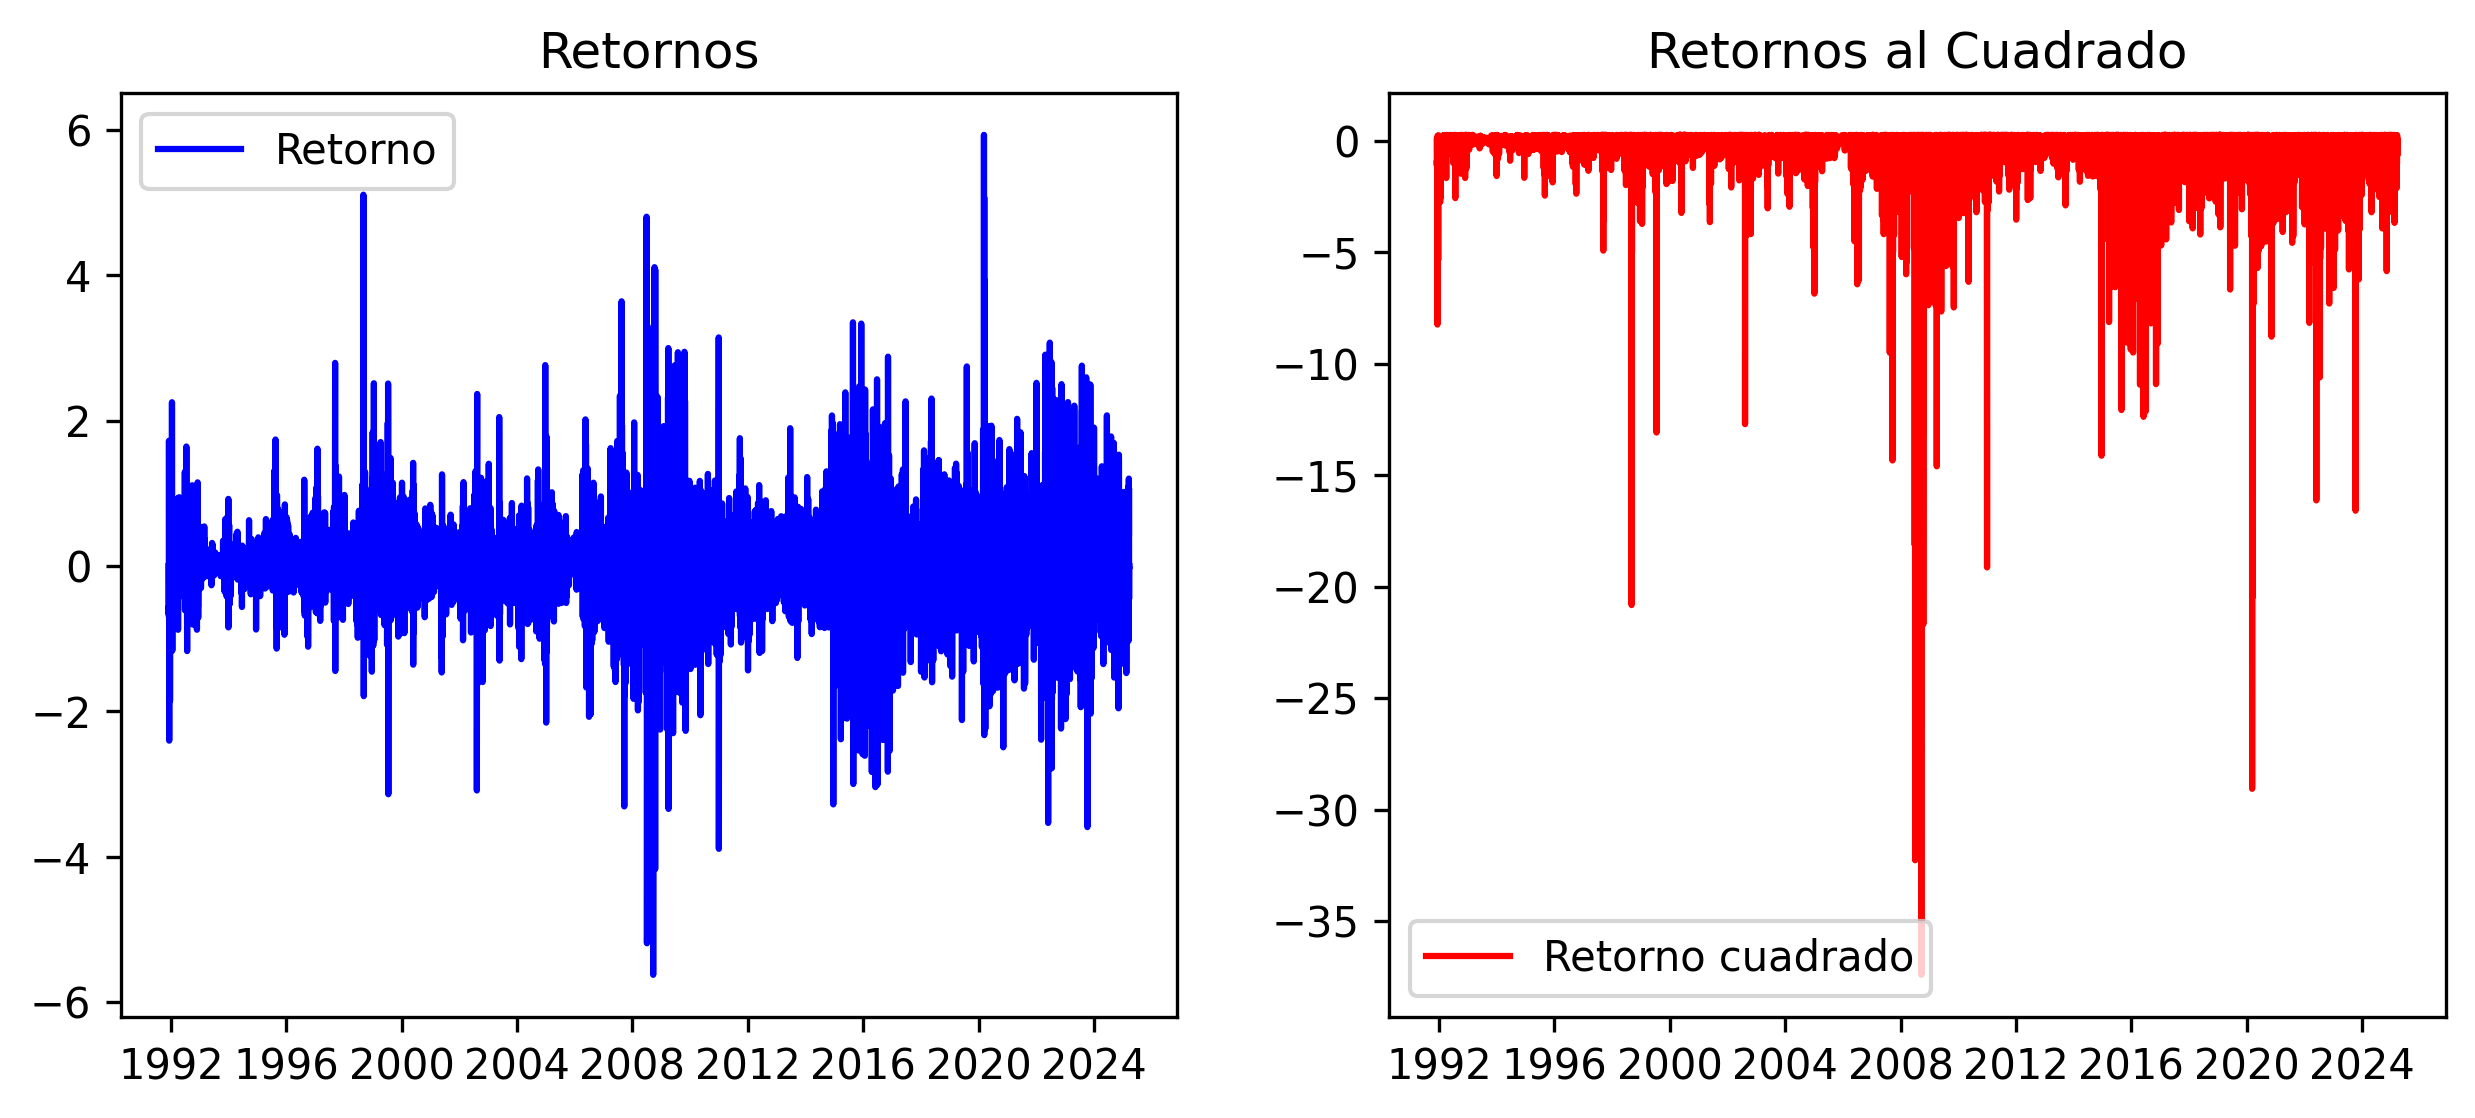
\includegraphics[width=0.9\linewidth]{output/subplot_retornos.png}
                \caption{Retornos}
                \label{fig:retornos}
            \end{figure}

En la gráfica de los retornos mensuales podemos observar que esta variable presenta alta volatilidad. Hay periodos de tiempo donde se comporta relativamente estable, manteniéndose cerca del cero, pero hay momentos en que presentan clusters de volatilidad. Esto mismo se puede observar en la gráfica de los retornos mensuales al cuadrado.
            
        \end{tcolorbox}
\end{enumerate}

{Ahora, asuman que los datos de los retornos mensuales $r_t$ tienen una estructura de la forma:}
\begin{align*}
    \Phi(L)r_t &= \Theta(L)\varepsilon_t \\
    \Phi(L) = 1 − \phi_1L &− \phi_2L^2 − \cdots − \phi_pL^p \\
    \Theta(L) = 1 + \theta_1L &+ \theta_2L^2 + \cdots + \theta_pL^p
\end{align*}

{Por su parte el error $\varepsilon_t$ puede seguir un ruido blanco fuerte ($\varepsilon_t\sim WN(0,
\sigma^2)$) o débil ($\varepsilon_t\sim D(0,\sigma_t^2)$).}

\begin{enumerate}[label = \emph{\alph*})]\setcounter{enumi}{3}
    \item {Estime el retorno mensual de la TRM que sigue un proceso ARMA. Justifique su estimaci\'on con estad\'isticas y criterios de informaci\'on.}
        \begin{tcolorbox}[title=Soluci\'on 2.d]
            \begin{table}[H]
\label{tab:dickey_fuller}
\centering
\begin{tabular}{lr}
\toprule
 & Valor \\
\midrule
Estad\'istico DF & -12.7408 \\
p-valor & 0.0000 \\
\bottomrule
\end{tabular}
\caption{Prueba Dickey-Fuller}
\end{table}

            \begin{figure}[H]
                \centering
                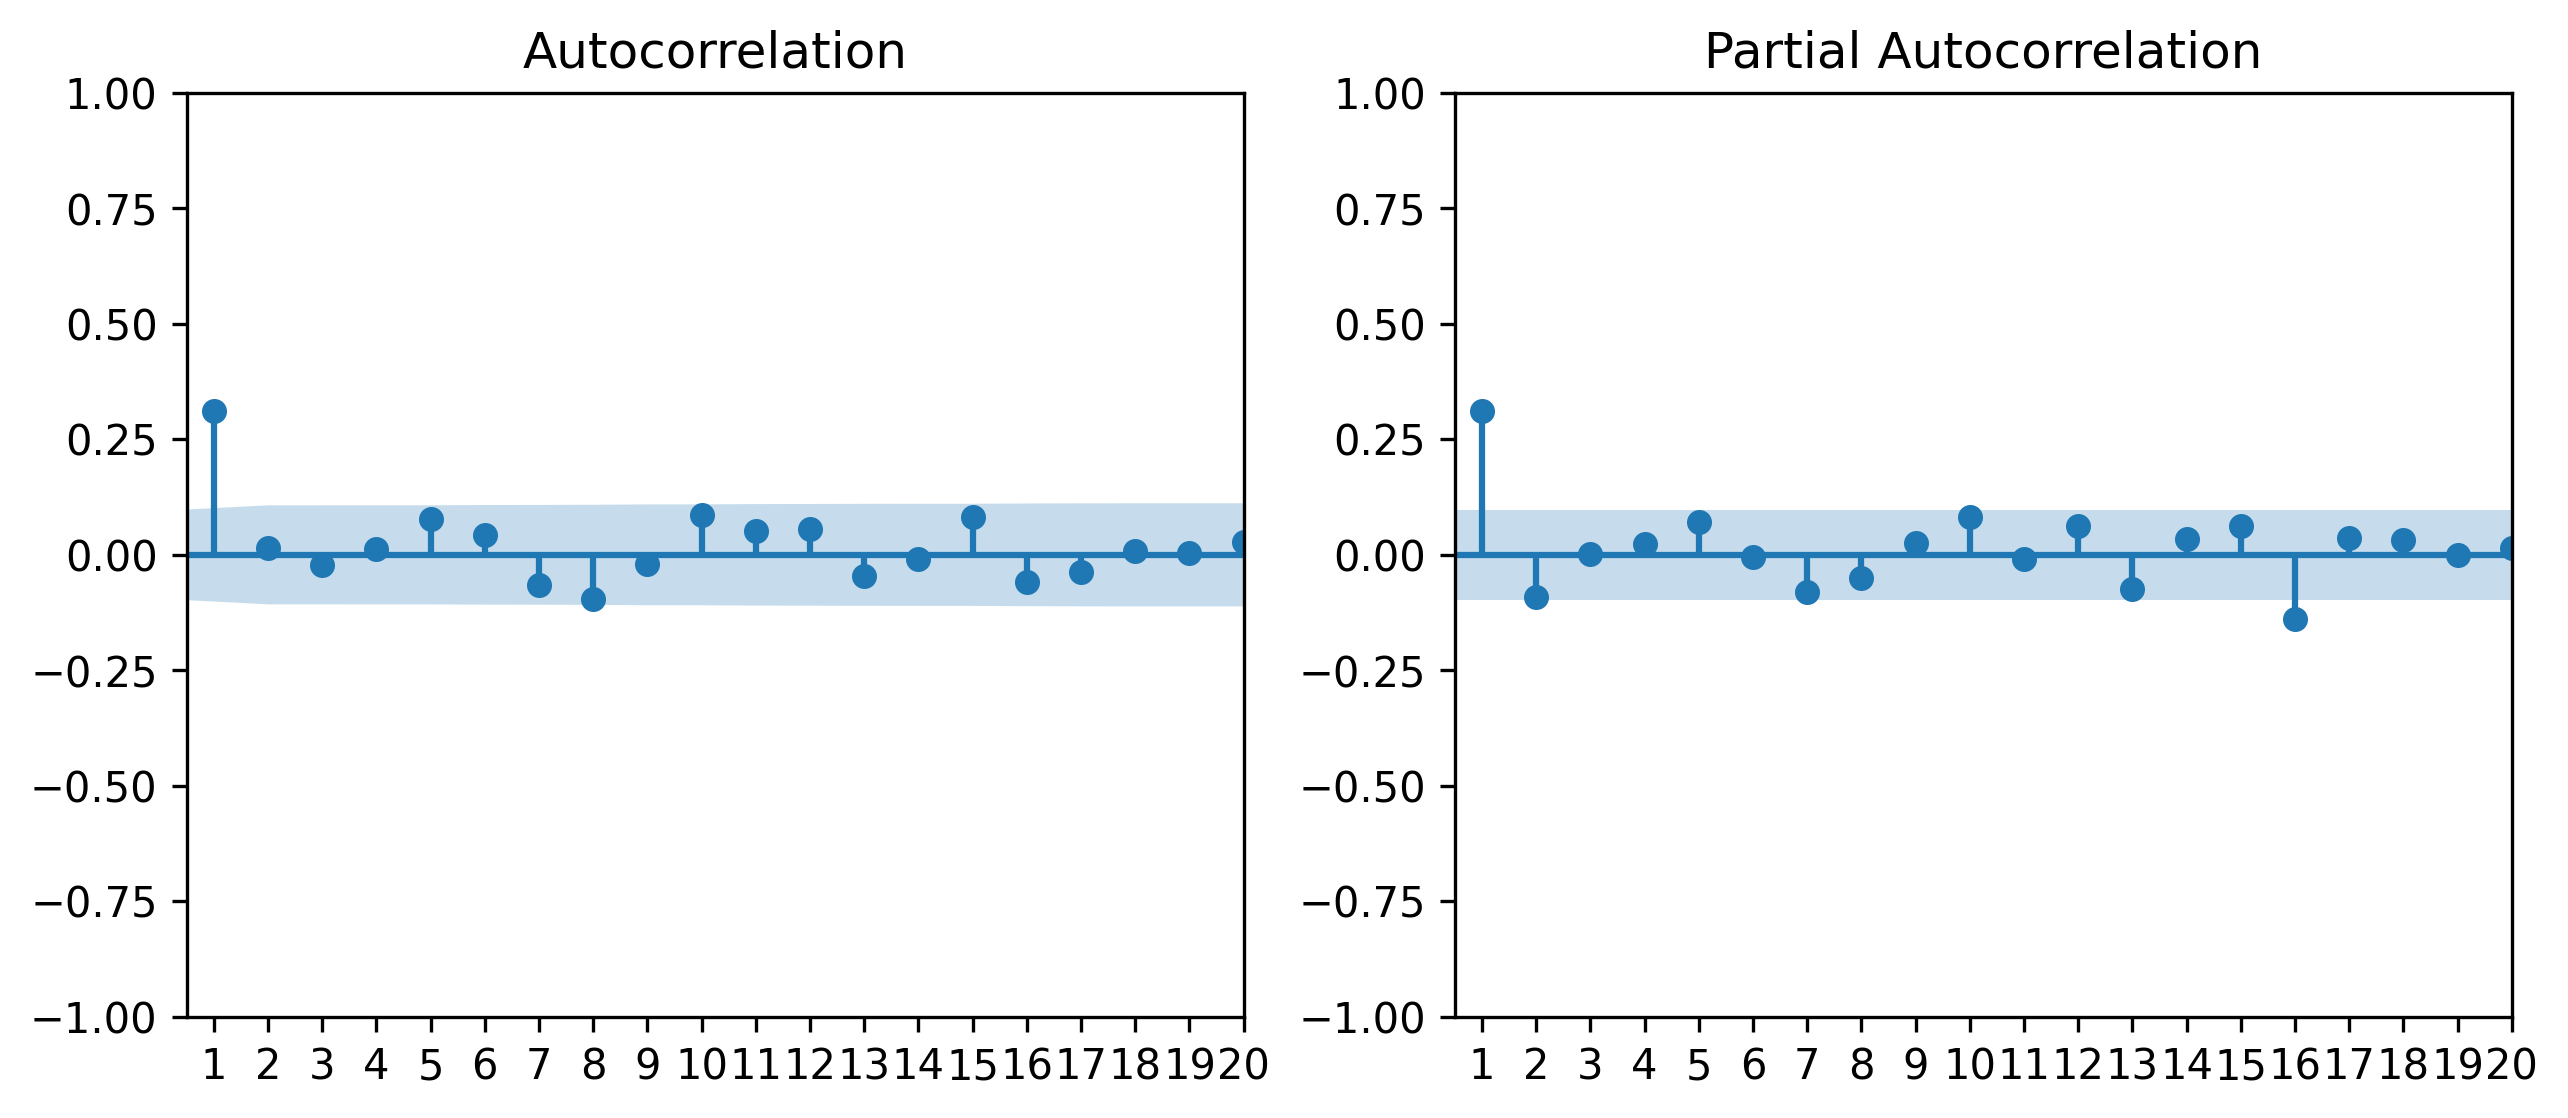
\includegraphics[width=0.9\linewidth]{output/acf_pacf_retornos.png}
                \caption{Autocorrelaciones de los Retornos Mensuales}
                \label{fig:corr_ret}
            \end{figure}
            \begin{table}[H]
\label{tab:autoarima_aic}
\centering
\begin{tabular}{rrrrr}
\toprule
0 & 1 & 2 & 3 & 4 \\
\midrule
1981.0158 & 1939.6620 & 1941.3115 & 1943.2209 & 1944.9339 \\
1942.4140 & 1941.3505 & 1943.2788 & 1945.1883 & 1946.8547 \\
1941.1070 & 1943.1068 & 1945.0487 & \textbf{1938.1438} & 1940.1096 \\
1943.1066 & 1945.1065 & 1941.6319 & 1940.1045 & 1944.7693 \\
1944.8736 & 1946.3898 & 1943.5636 & 1945.6314 & 1945.1468 \\
\bottomrule
\end{tabular}
\caption{Criterio AIC}
\end{table}

            \begin{table}[H]
\label{tab:autoarima_bic}
\centering
\begin{tabular}{rrrrr}
\toprule
0 & 1 & 2 & 3 & 4 \\
\midrule
1981.0158 & 1939.6620 & 1941.3115 & 1943.2209 & 1944.9339 \\
1942.4140 & 1941.3505 & 1943.2788 & 1945.1883 & 1946.8547 \\
1941.1070 & 1943.1068 & 1945.0487 & 1938.1438 & 1940.1096 \\
1943.1066 & 1945.1065 & 1941.6319 & 1940.1045 & 1944.7693 \\
1944.8736 & 1946.3898 & 1943.5636 & 1945.6314 & 1945.1468 \\
\bottomrule
\end{tabular}
\caption{Criterio BIC}
\end{table}


Dados los criterios AIC y BIC calculados, el retorno mensual de la TRM puede seguir un proceso ARMA(2,3) (pues el criterio de AIC para este modelo es el menor), o un proceso ARMA(0,1) (pues el criterio BIC para este modelo es el menor). Para escoger el modelo apropiado, seguimos el criterio de parsimonia: escogemos el modelo más simple, el ARMA(0,1).

   
        \end{tcolorbox}

    \item {Construya y grafique la serie de residuales. Justifique que se trata de ruido blanco. Documente pruebas de normalidad y aquellas relevantes para justificar los supuestos de su modelo.}
        \begin{tcolorbox}[title=Soluci\'on 2.e]
            \begin{figure}[H]
                \centering
                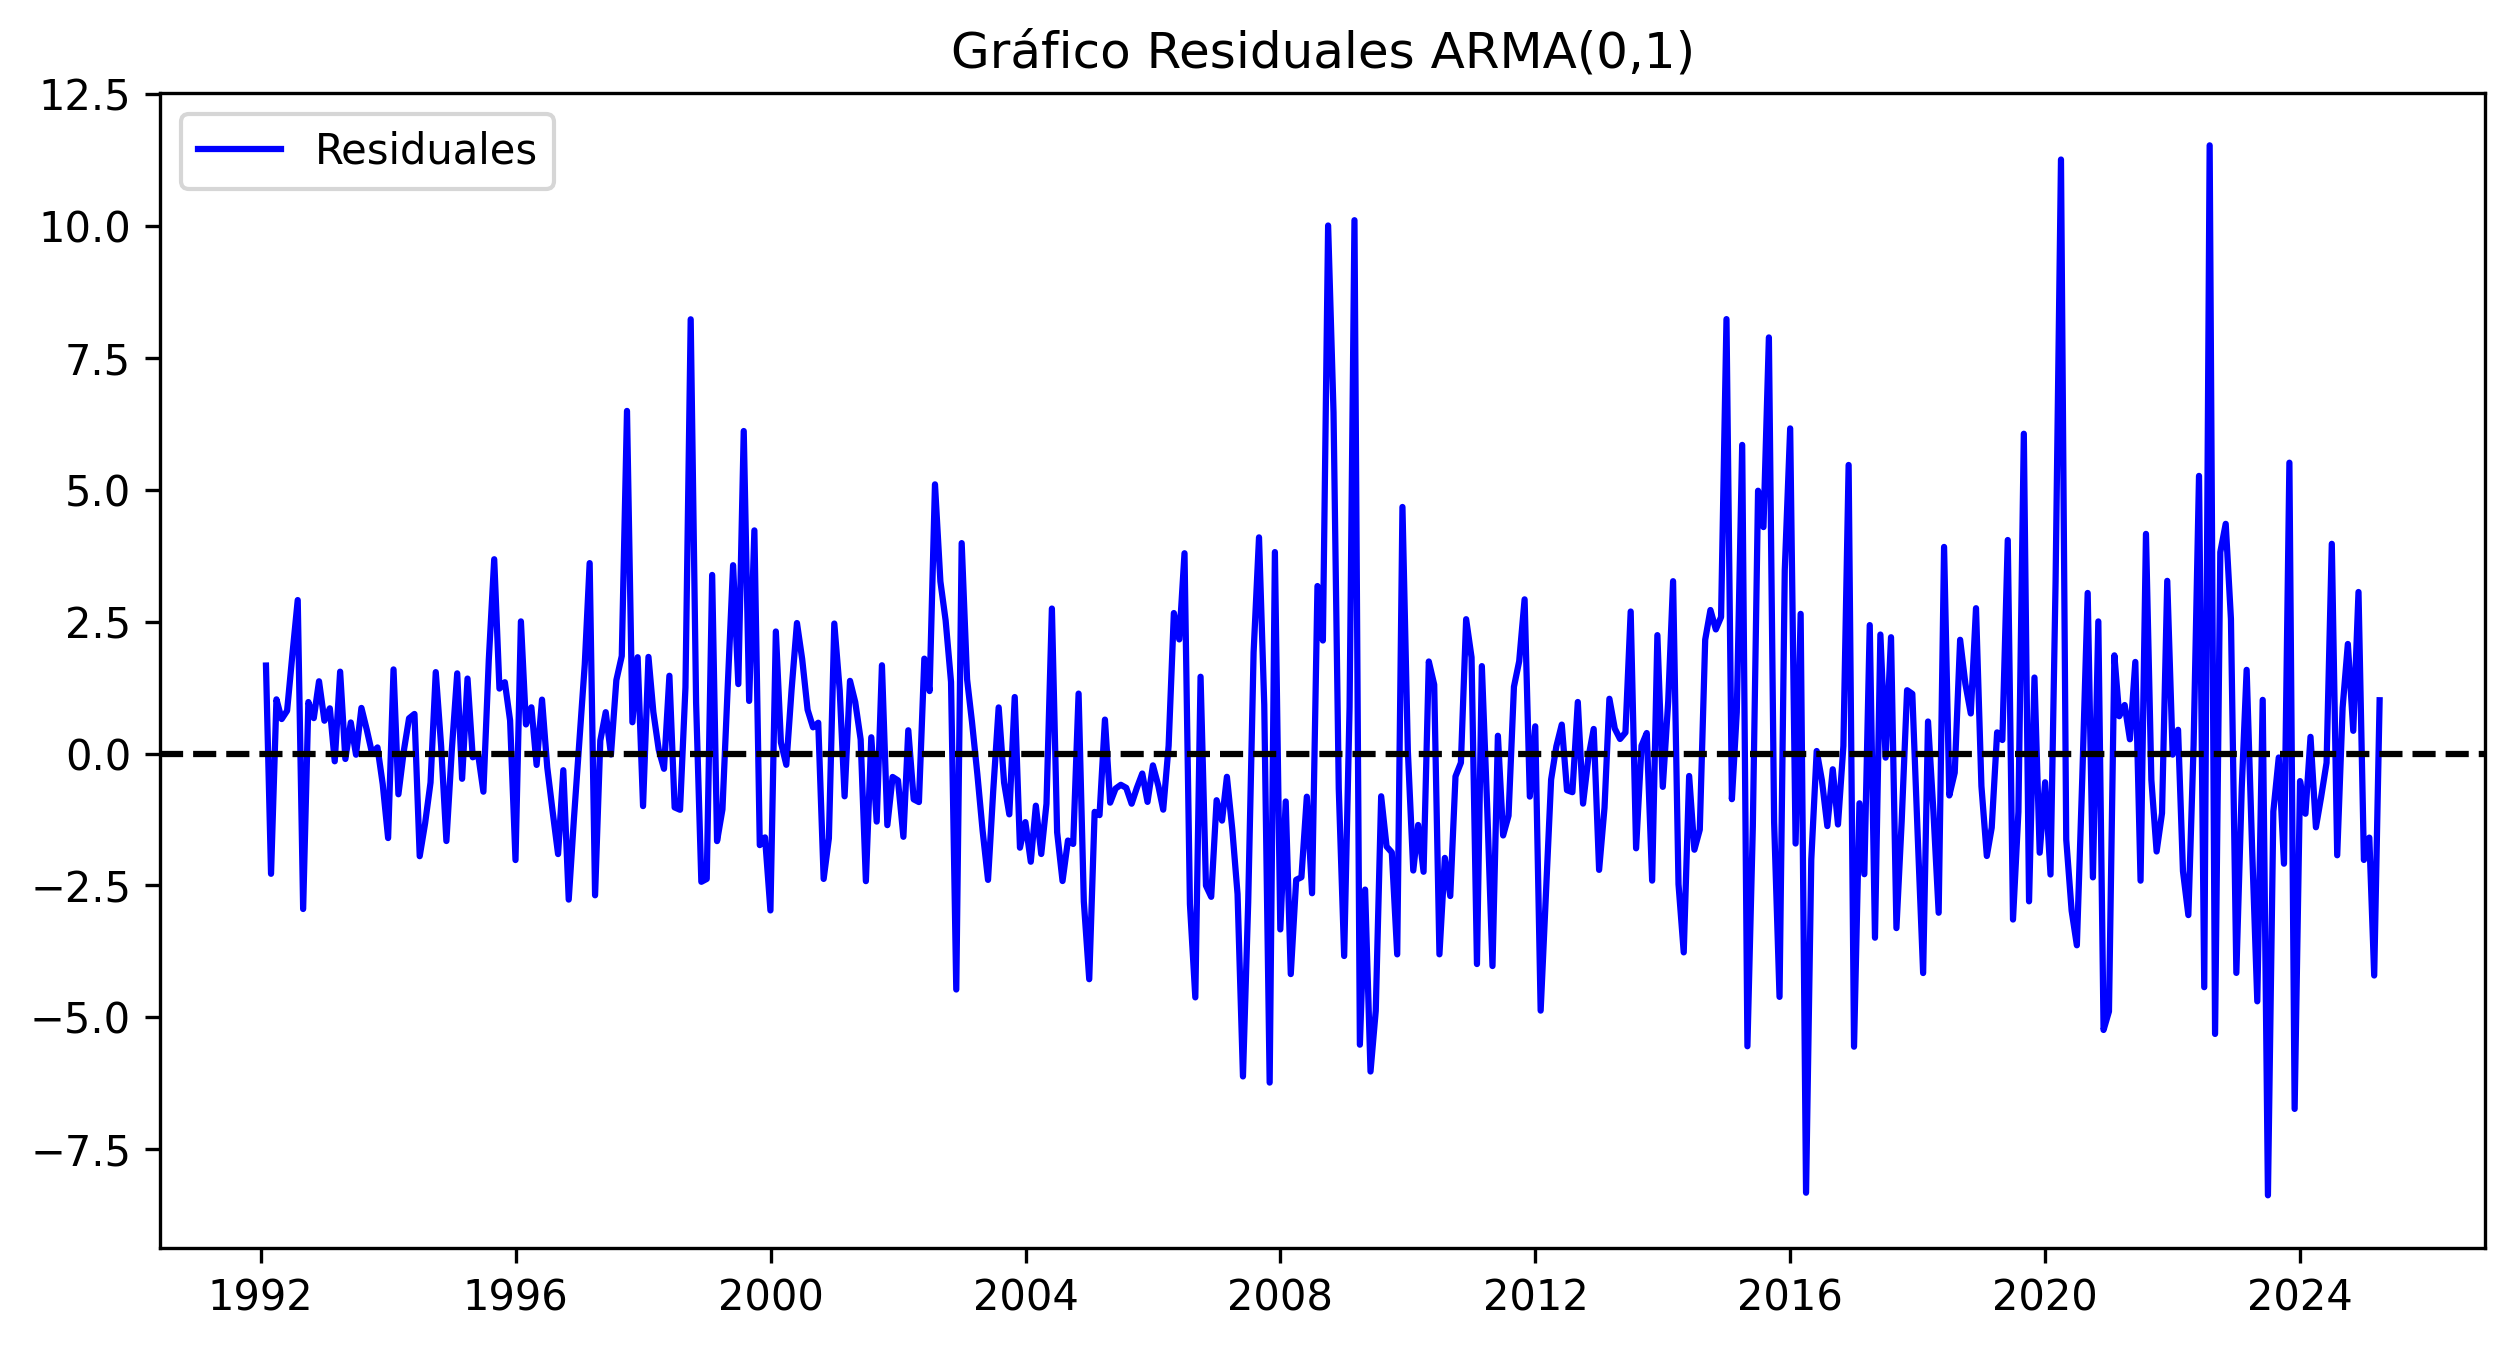
\includegraphics[width=0.9\linewidth]{output/graf_resid.png}
                \caption{Gr\'afico de los Residuales del modelo ARMA(0,1)}
                \label{fig:residuales}
            \end{figure}
             \begin{figure}[H]
                \centering
                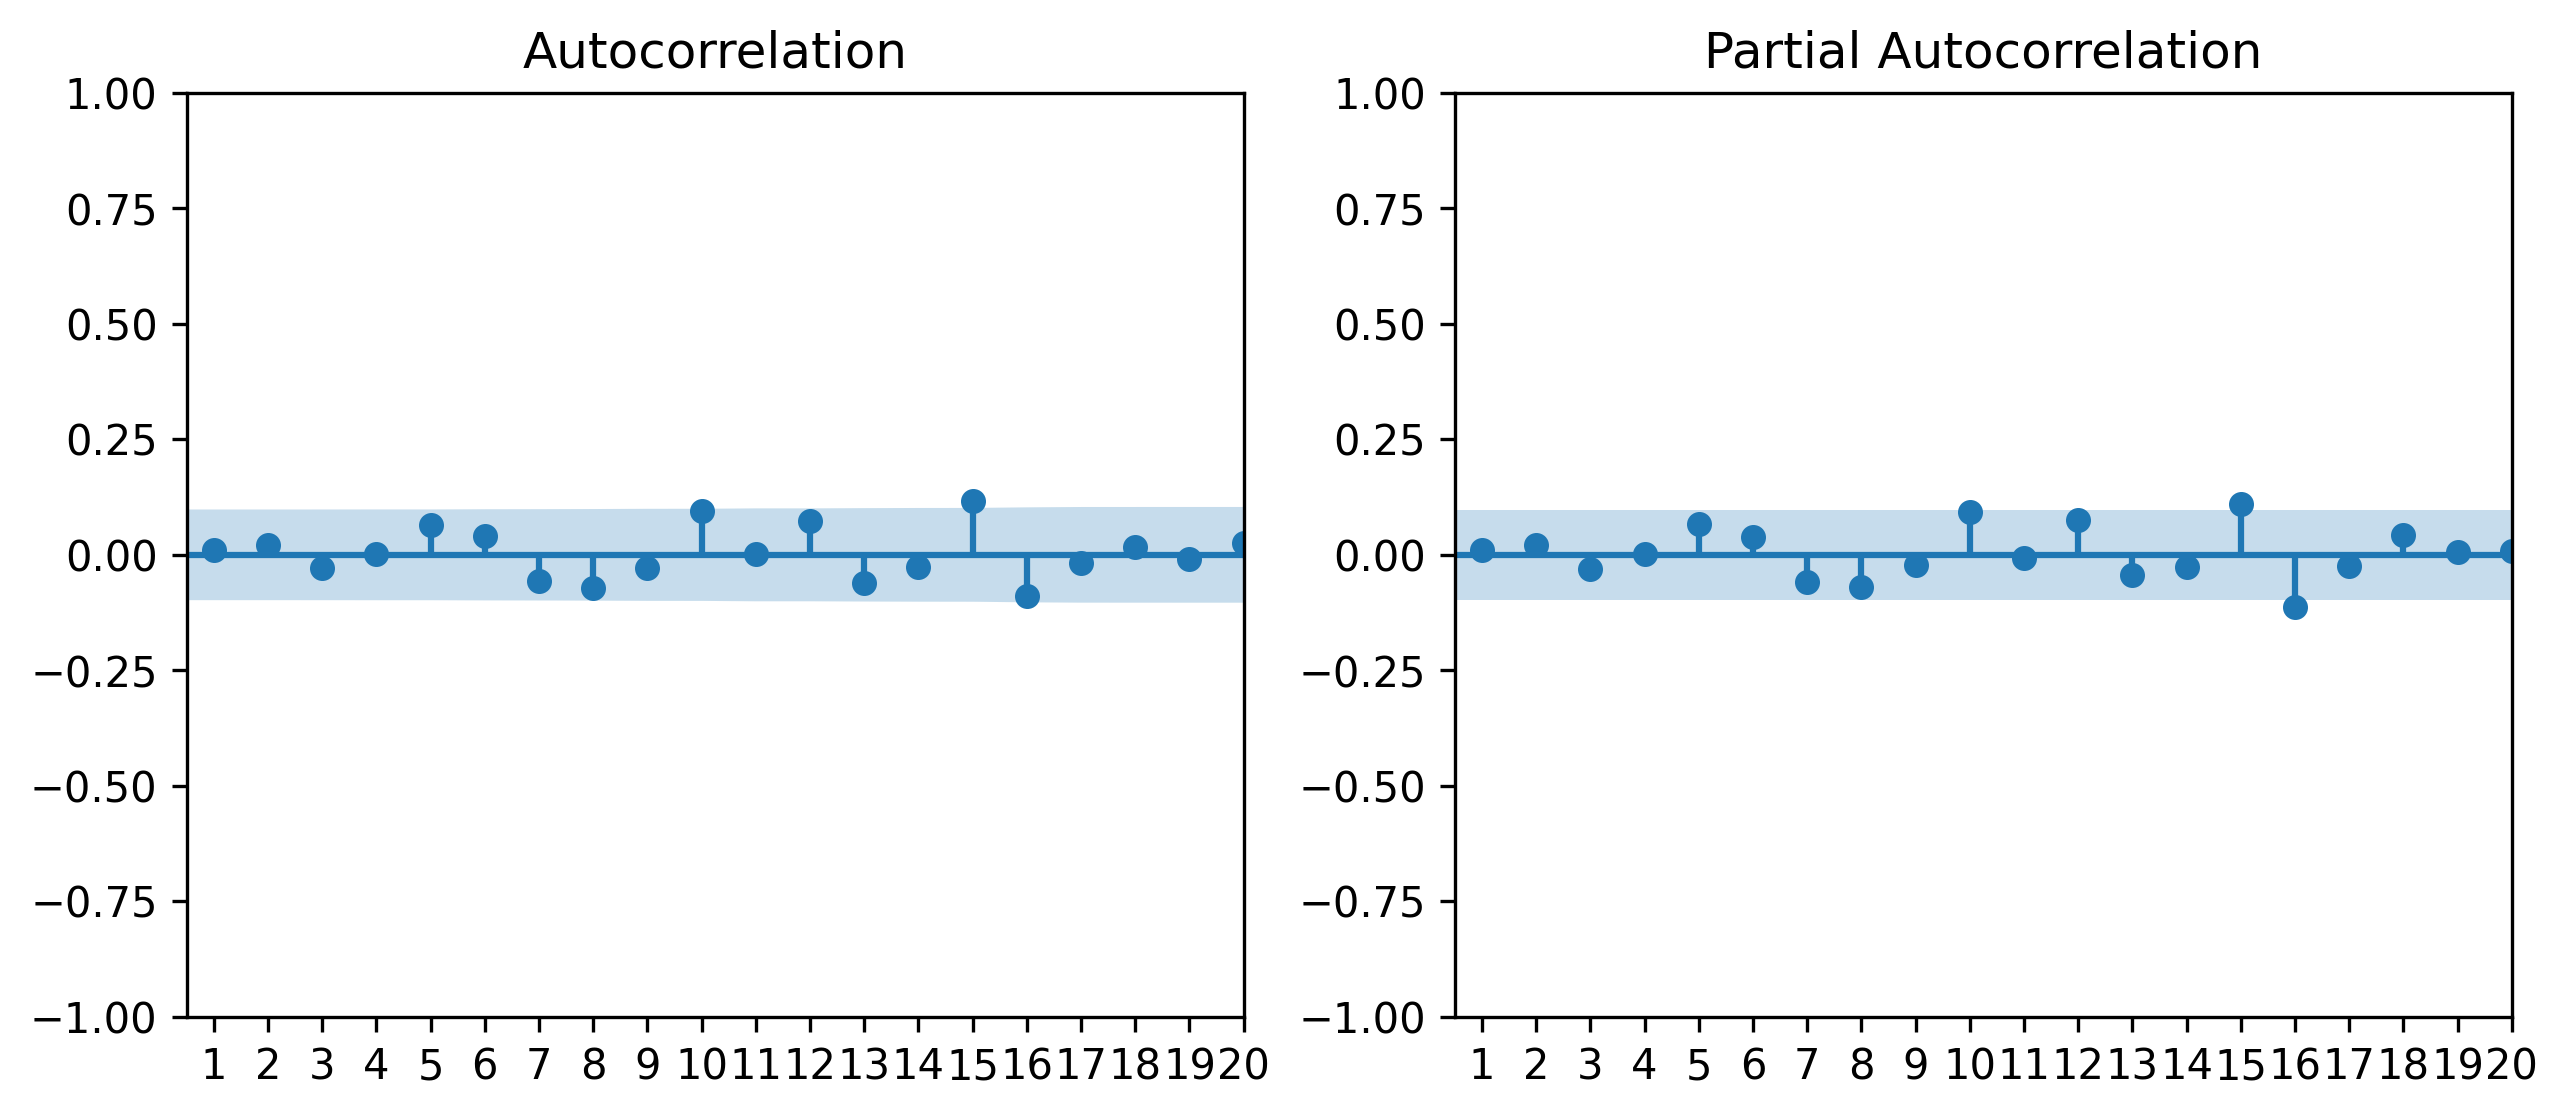
\includegraphics[width=0.9\linewidth]{output/acf_pacf_residuales.png}
                \caption{Autocorrelaciones de los Residuales del modelo ARMA(0,1)}
                \label{fig:corr_resid}
            \end{figure}

            \begin{table}[H]
\label{tab:q_test_resid}
\centering
\begin{tabular}{lrr}
\toprule
 & Estad\'istico & P-Valor \\
\midrule
5 & 2.2927 & 0.8073 \\
10 & 10.3611 & 0.4094 \\
15 & 20.1167 & 0.1675 \\
\bottomrule
\end{tabular}
\caption{Prueba Q Residuales}
\end{table}

            
            \begin{figure}[H]
                \centering
                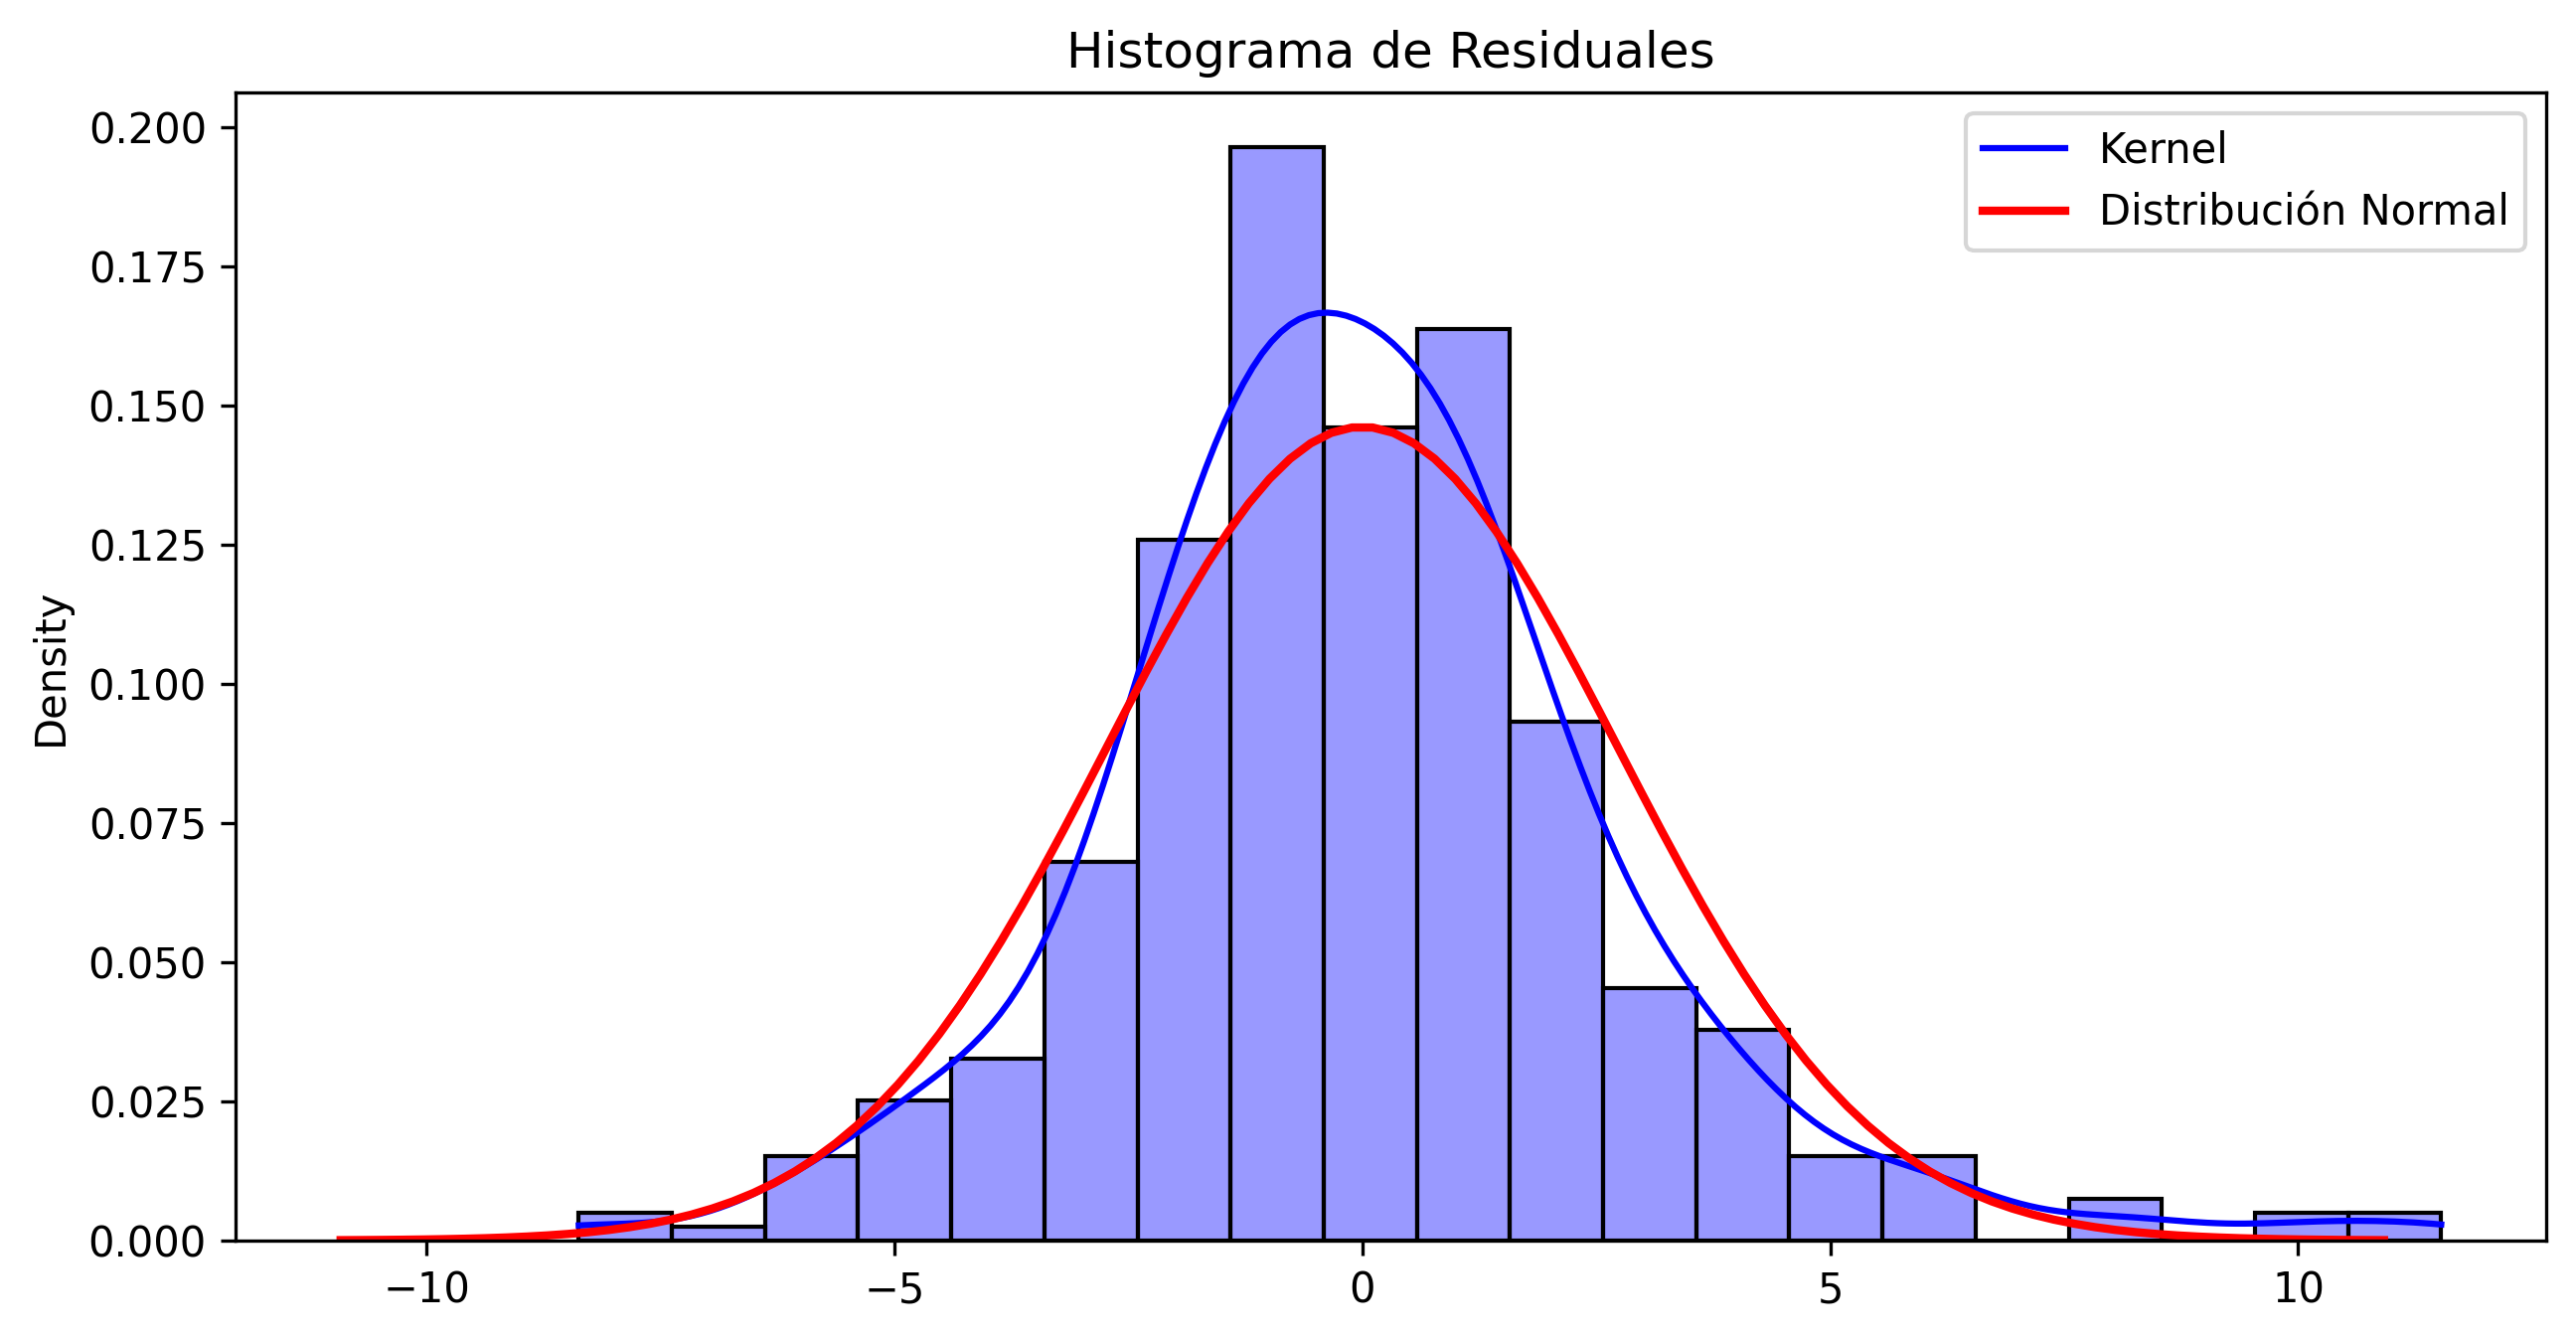
\includegraphics[width=0.9\linewidth]{output/hist_resid.png}
                \caption{Histograma de los Residuales del modelo ARMA(0,1)}
                \label{fig:hist_resid}
            \end{figure}
            \begin{figure}[H]
                \centering
                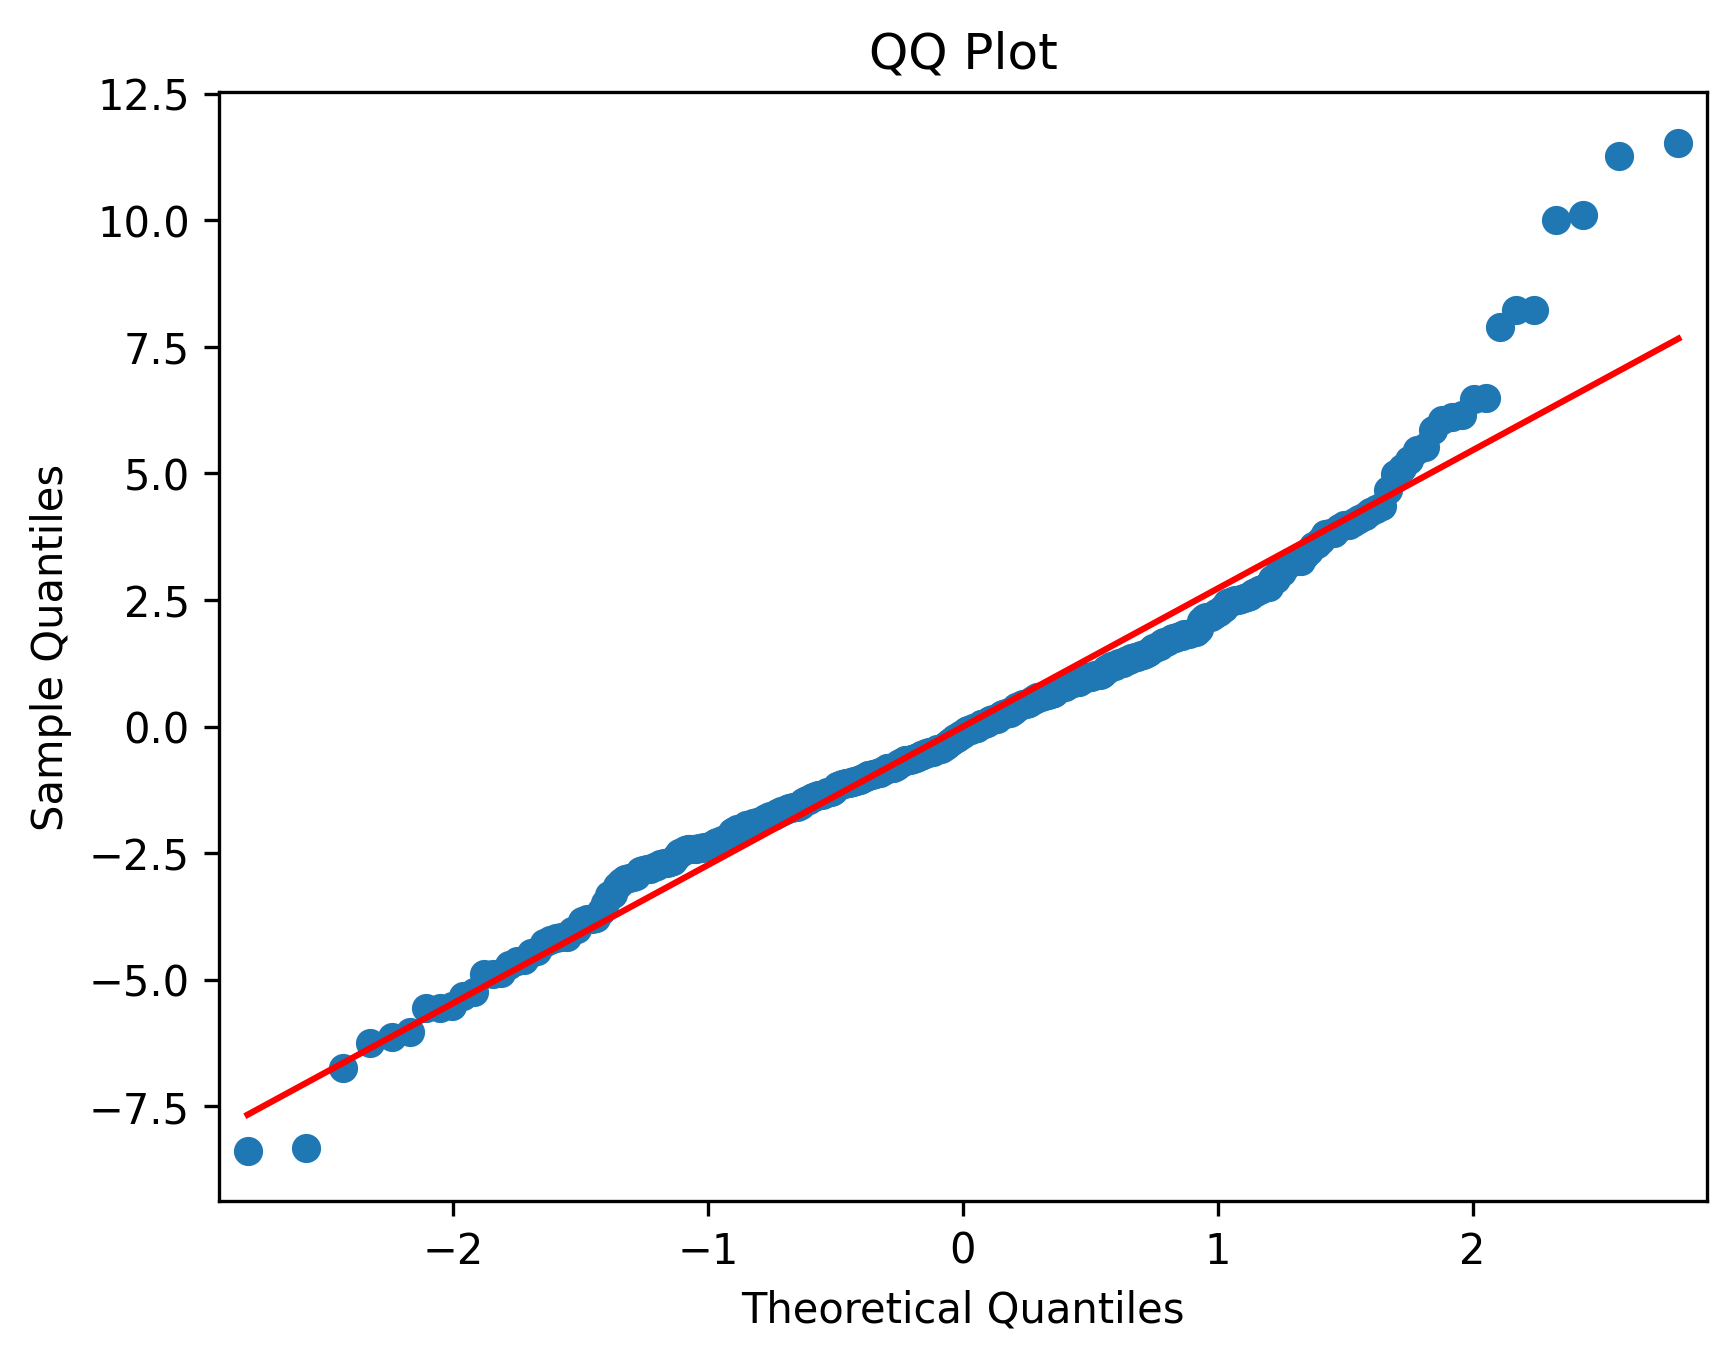
\includegraphics[width=0.7\linewidth]{output/qq_plot_residuales.png}
                \caption{QQ-Plot de los Residuales del modelo ARMA(0,1)}
                \label{fig:qq_resid}
            \end{figure}

Al observar la gráfica de los residuales del modelo, se puede apreciar que no hay ningún comportamiento predecible  ni tendencias. Los autocorrelogramas hacen esto igual de evidente. La prueba de Ljung-Box hace claro que no hay autocorrelación estadísticamente significativa, es decir, no se rechaza que la serie de los residuales se comporta como ruido blanco. Adicionalmente, el histograma de los residuales muestra que la distribución de estos se aproxima a una distribución normal estándar.
        \end{tcolorbox}
    \item {Pruebe si es necesario incluir din\'amicas de varianza condicional. De ser necesario, est\'imelas y presente sus resultados (puede probar varios modelos, pero debe presentar y continuar el desarrollo del taller con uno solo). Justifique con estad\'isticas y criterios de informaci\'on el modelo estimado.}
        \begin{tcolorbox}[title=Soluci\'on 2.f]
            \begin{figure}[H]
                \centering
                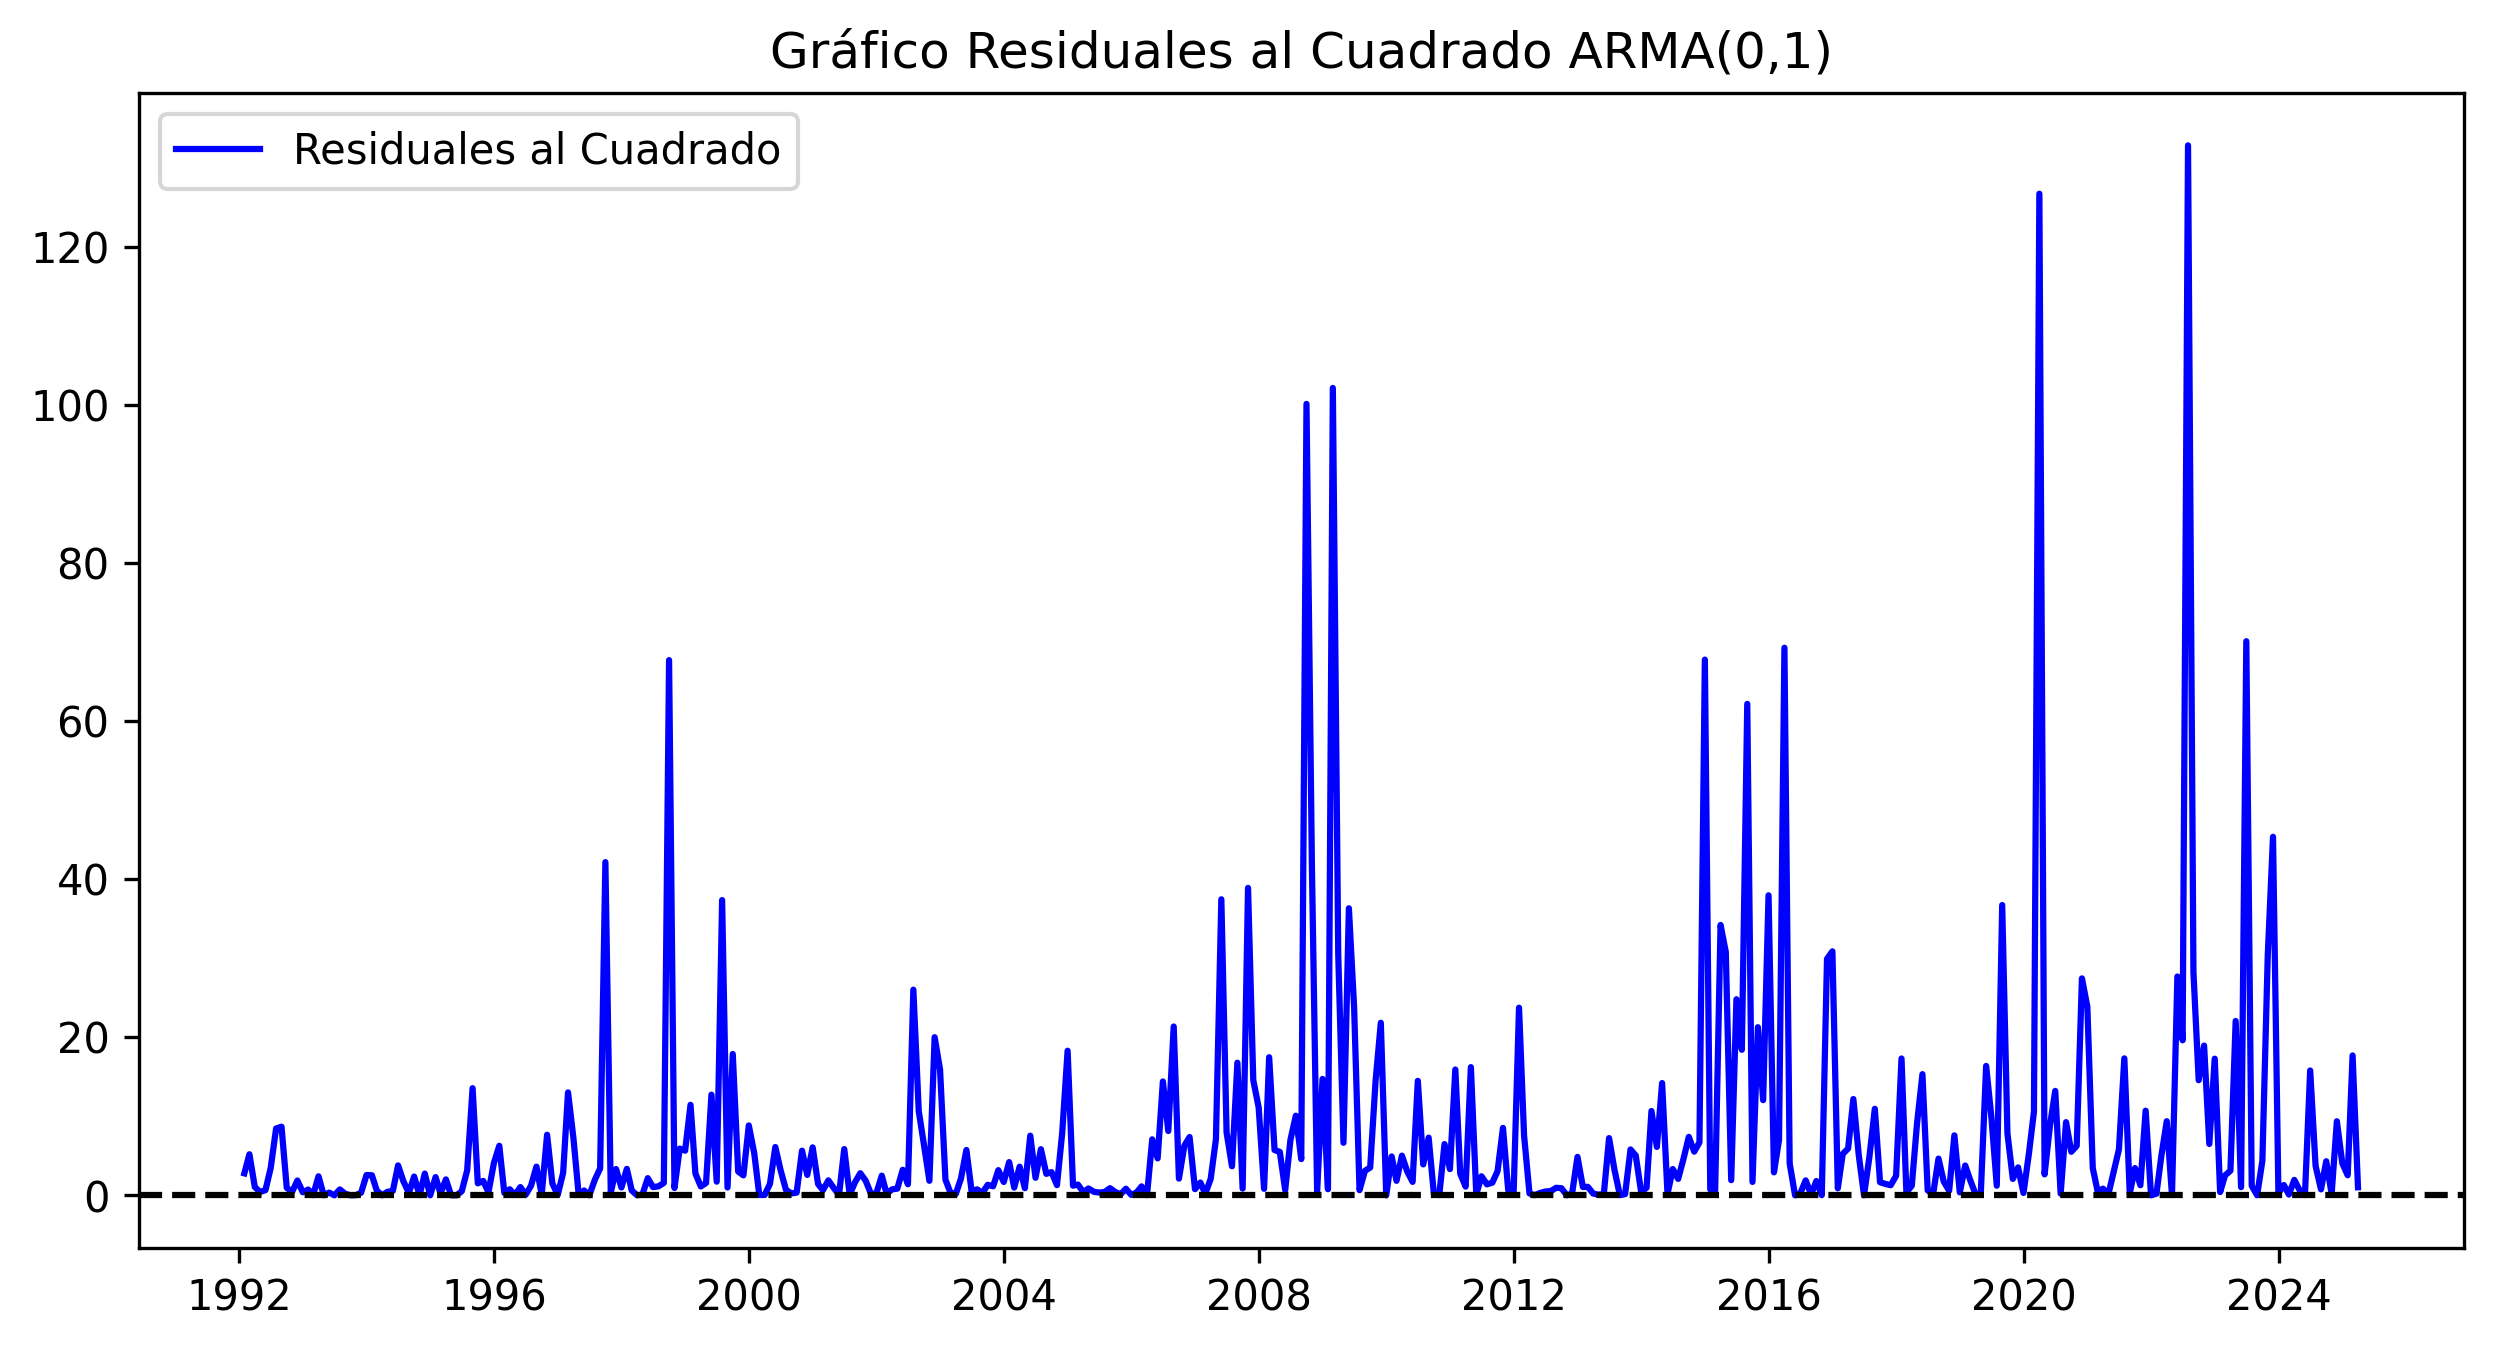
\includegraphics[width=0.9\linewidth]{output/graf_resid2.png}
                \caption{Gr\'afica de Residuales al Cuadrado del modelo ARMA(0,1)}
                \label{fig:graf_resid2}
            \end{figure}
            
            \begin{figure}[H]
                \centering
                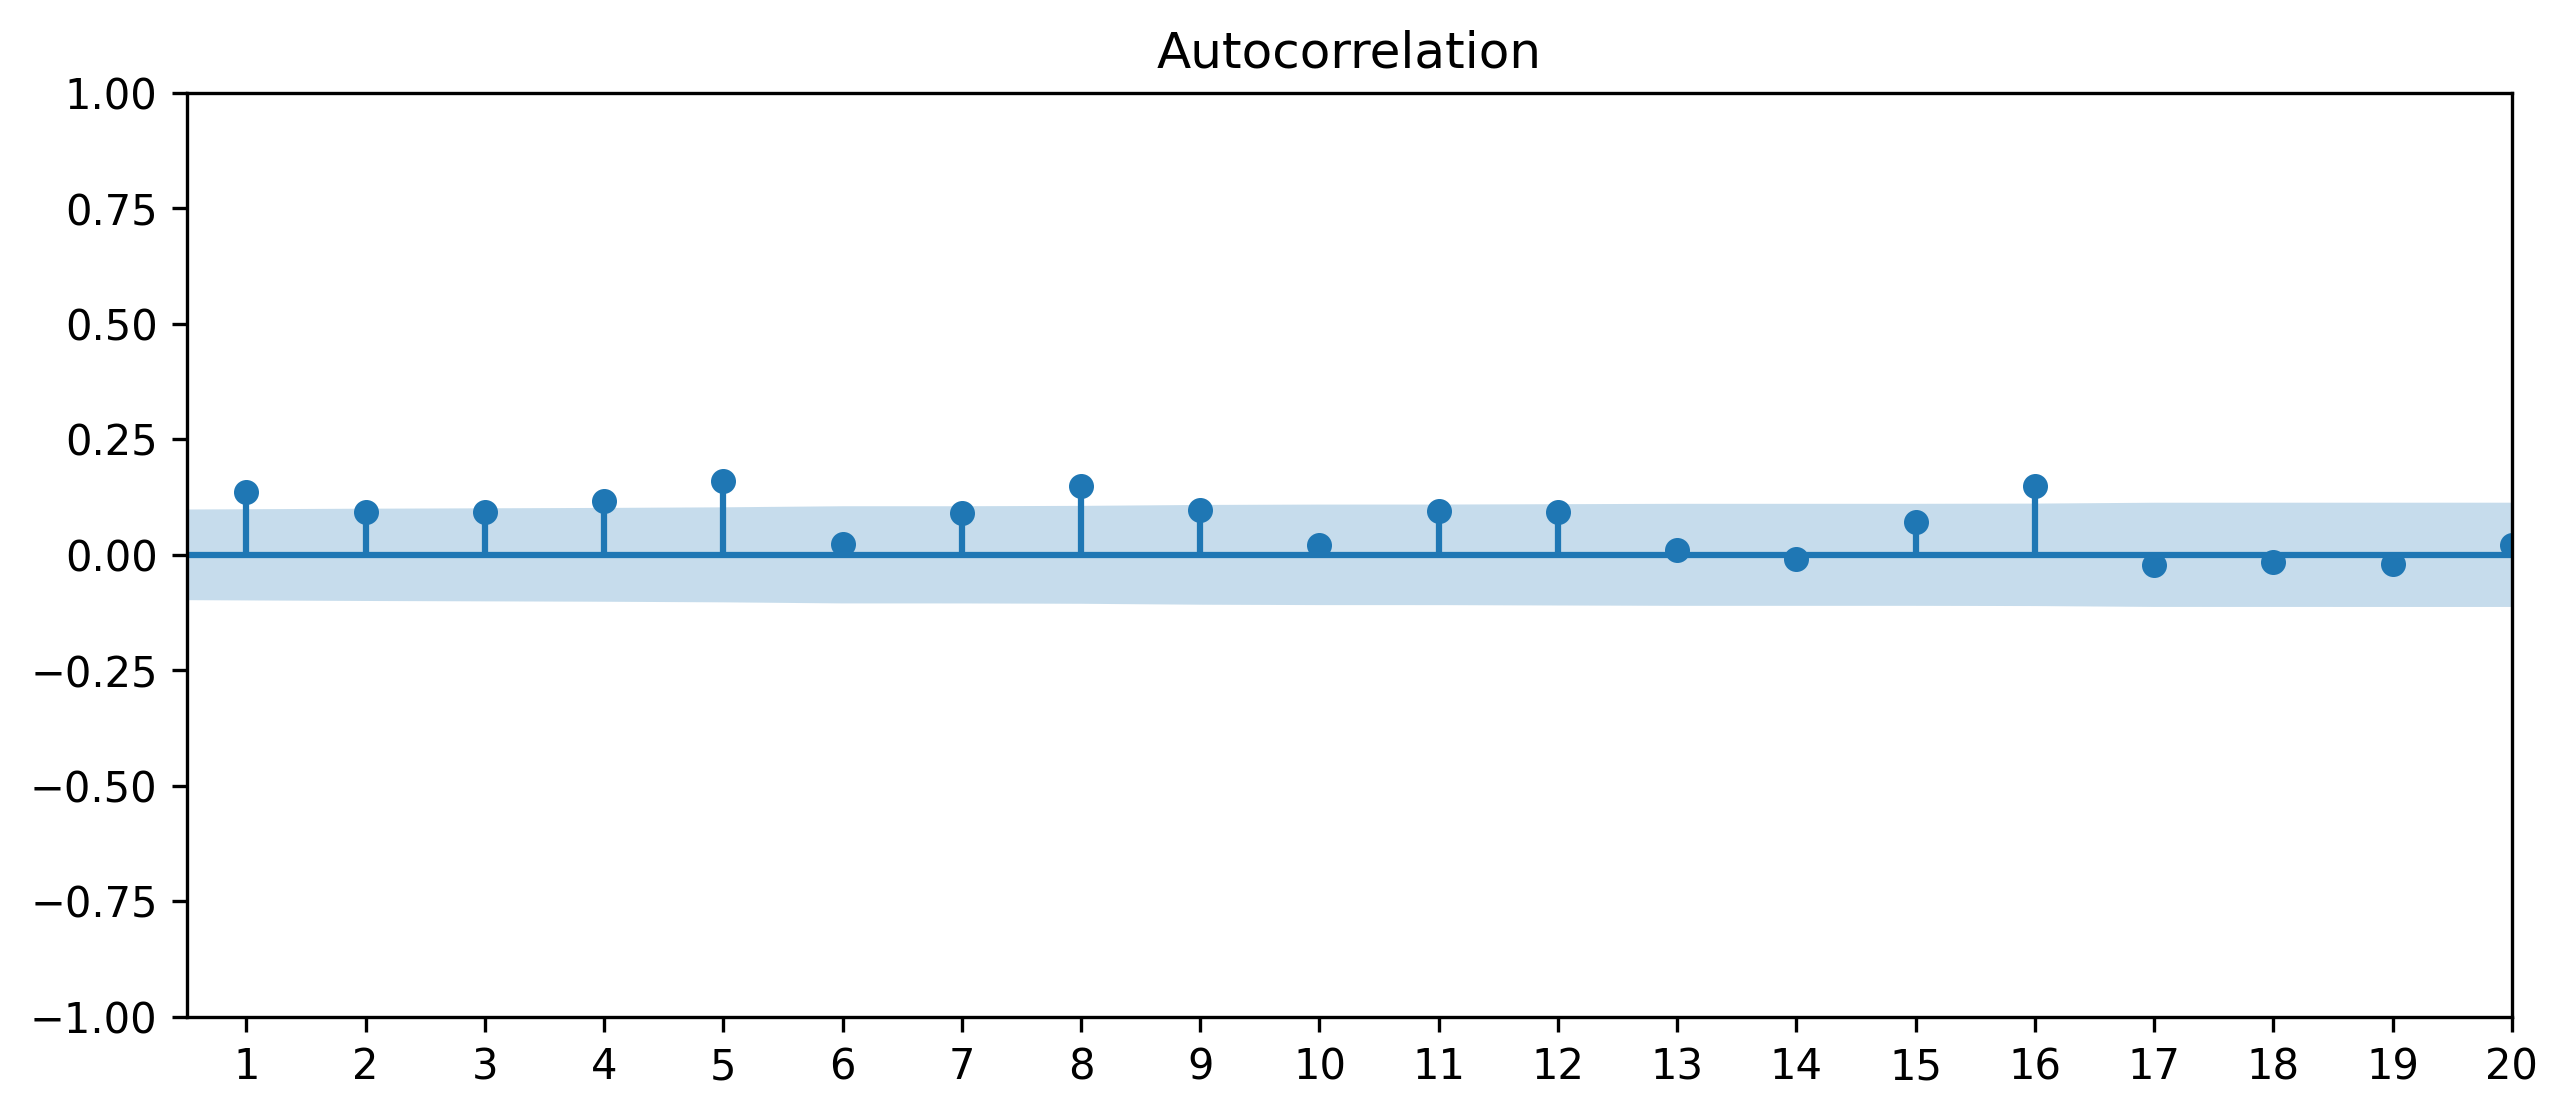
\includegraphics[width=0.9\linewidth]{output/acf_residuales2.png}
                \caption{Autocorrelaci\'on Residuales al Cuadrado}
                \label{fig:acf_resid2}
            \end{figure}

            \begin{table}[H]
\label{tab:q_test_resid2}
\centering
\begin{tabular}{lrr}
\toprule
 & Estad\'istico & P-Valor \\
\midrule
5 & 30.1437 & 0.0000 \\
10 & 46.8140 & 0.0000 \\
15 & 56.4281 & 0.0000 \\
\bottomrule
\end{tabular}
\caption{Prueba Q Residuales al Cuadrado}
\end{table}

        \end{tcolorbox}
    \item {Pruebe si su modelo captura correctamente las din\'amicas de varianza. Realice y documente las pruebas necesarias.}
        \begin{tcolorbox}[title=Soluci\'on 2.g]
            \begin{figure}[H]
                \centering
                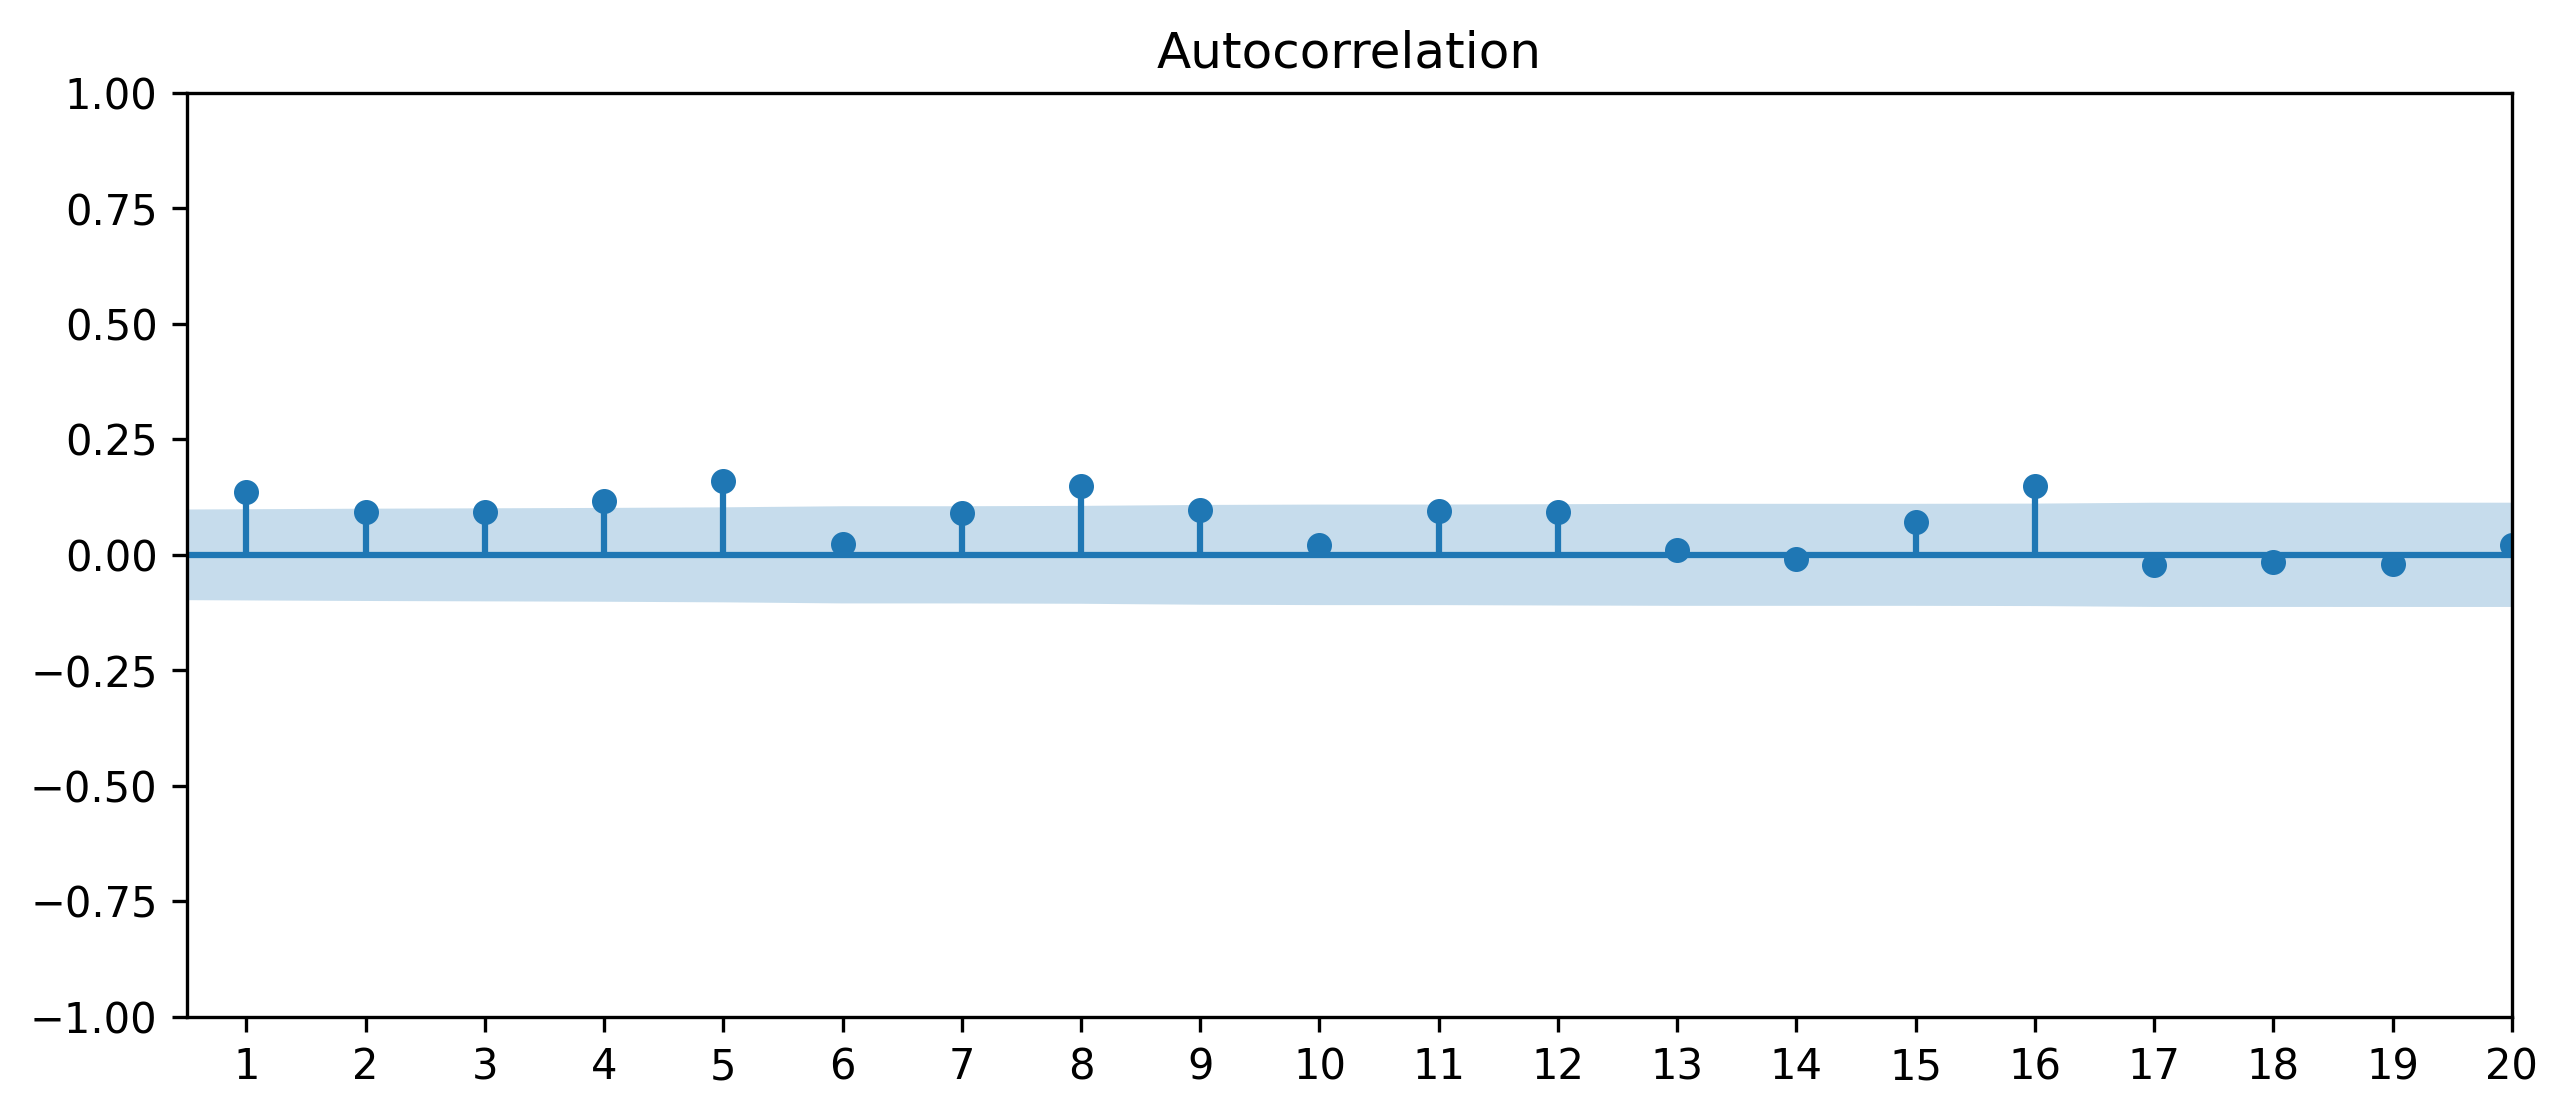
\includegraphics[width=0.9\linewidth]{output/acf_residuales2.png}
                \caption{Autocorrelaci\'on Residuales al Cuadrado}
                \label{fig:acf_resid2}
            \end{figure}
        \end{tcolorbox}
\end{enumerate}

{A usted le encanta viajar y entiende que cuando viaja al exterior su plan de vacaciones puede salir m\'as caro o m\'as barato dependiendo la TRM (en este caso retornos positivos jugar\'ian en su contra). Usted tiene $\$20.000.000$ ahorrados que est\'a dispuesto a gastarse en un fant\'astico viaje a la ciudad maravilla, pero no sabe si adquirir todo lo relacionado con el viaje en este momento o esperar hasta el primer d\'ia de mayo. Afortunadamente, usted est\'a tomando el curso de pron\'osticos y acaba de estimar un modelo que le sirve para pronosticar los retornos mensuales de la TRM y su volatilidad, lo que le ayudar\'a a tomar una decisi\'on.}

\begin{enumerate}[label = \emph{\alph*})]\setcounter{enumi}{7}
    \item {Realice el pron\'ostico punto para abril del año 2025 tanto de los retornos como de la varianza. Reporte el pron\'ostico para los dos casos e interprete los dos resultados (no se pide realizar el pronostic\'o a mano, puede usar los comandos necesarios para realizar el pron\'ostico 1 paso adelante).}
        \begin{tcolorbox}[title=Soluci\'on 2.h]
            
        \end{tcolorbox}
    \item {Con el comando apropiado simule mil pron\'osticos del retorno mensual de la TRM para el mes de abril del año 2025. Haga una gr\'afica con su estimaci\'on puntual y con la funci\'on de densidad generada a partir de simulaciones de su modelo autoregresivo de media m\'ovil, indique en la gr\'afica el intervalo del 95\% de confianza: ¿Seg\'un su pron\'ostico, para el mes de abril del año 2025, ser\'ia mejor comprar todo lo relacionado con su viaje hoy o esperar el mes de abril? ¿Con los retornos esperados pronosticados usted espera una apreciaci\'on o una depreciaci\'on del peso frente al d\'olar?}
        \begin{tcolorbox}[title=Soluci\'on 2.i]
            
        \end{tcolorbox}
    \item {Ahora, todos los valores pronosticados de los retornos de la TRM para el mes de abril del año 2025 calculados en el item anterior, multipl\'iquelos por $\$20.000.000$, con esto obtendr\'a un vector de lo que ganar\'ia (si hay apreciaci\'on) y lo que perder\'ia (si hay depreciaci\'on) si decide esperar un mes y comprar todo lo relacionado con su viaje. Haga una gr\'afica con su estimaci\'on puntual y con la funci\'on de densidad generada a partir de las estimaciones, indique en la gr\'afica el intervalo del 95\% de confianza: ¿Seg\'un su pron\'ostico, usted esperar\'ia o mejor comprar\'ia todo lo relacionado con su viaje en este momento? ¿Teniendo en cuenta todo lo anterior invertir\'ia su dinero en activos asociados a la TRM peso d\'olar? ¿usar\'ia estos modelos para tomar este tipo de decisiones o mejor se guiar\'ia en su experiencia previa como turista?}
        \begin{tcolorbox}[title=Soluci\'on 2.j]
            
        \end{tcolorbox}
\end{enumerate}

\section{[45 puntos] Juntando Componentes.}

{Ahora debe pronosticar las remesas de los trabajadores trimestrales en pesos colombianos. Para esto, asuma que las series pueden seguir el modelo general visto en clase que incluye tendencia, estacionalidad, ciclos y din\'amicas de varianza.}

\begin{align*}
    y_t = T_t(\theta) +& \sum_{i=1}^{s} \gamma_i D_{it} + \varepsilon_t \\
    \Phi(L) \varepsilon_t =& \Theta(L) v_t \\
    \Phi(L) = 1 - \phi_1 L -& \phi_2 L^2 - \dots - \phi_p L^p \\
    \Theta(L) = 1 + \theta_1 L +& \theta_2 L^2 + \dots + \theta_p L^p
\end{align*}

{Por su parte el error $v_t$ puede seguir un ruido blanco fuerte ($v_t\sim WN(0,
\sigma^2)$) o d\'ebil ($v_t\sim D(0,\sigma_t^2)$).} \\

{En el archivo de Excel denominado remesas que acompaña este taller se encuentra una serie trimestral de las remesas en millones de d\'olares desde el primer trimestre del año 2000 hasta el cuarto trimestre de 2025.}

\begin{enumerate}[label=\emph{\alph*})]
    \item {Convierta los valores en d\'olares a valores en pesos, multiplic\'andolo por la TRM trimestral promedio de cada trimestre. Grafique los datos trimestrales obtenidos en pesos. Describa la din\'amica de las series trimestrales de las remesas que ustedes construyeron que est\'an denominadas en pesos colombianos. ¿Observan un cambio de tendencia de la serie a trav\'es del tiempo? Escriban expl\'icitamente si los datos trimestrales est\'an en millones de pesos, en miles de millones de pesos o en billones de pesos.}
        \begin{tcolorbox}[title=Soluci\'on 3.a]
        La serie trimestral del logaritmo de las remesas en millones de pesos colombianos presentó un crecimiento sostenido desde el año 2000 hasta el año 2005, alcanzando valores de casi 14.5 aproximadamente. Posterior a este periodo, las remesas presentaron un estancamiento alrededor de este valor, acompañado por caídas y subidas breves. Sin embargo, a partir del 2015, se presentó una notoria recuperación de la serie, donde las remesas presentaron un crecimiento acelerado y constante alcanzando valores máximos superiores a 16 a finales del 2024. Por otro lado, se observa que la serie tiene, en su mayoría, una tendencia positiva creciente. Finalmente, los datos se encuentran en millones de pesos colombianos. 
\begin{figure}[H]
    \centering
    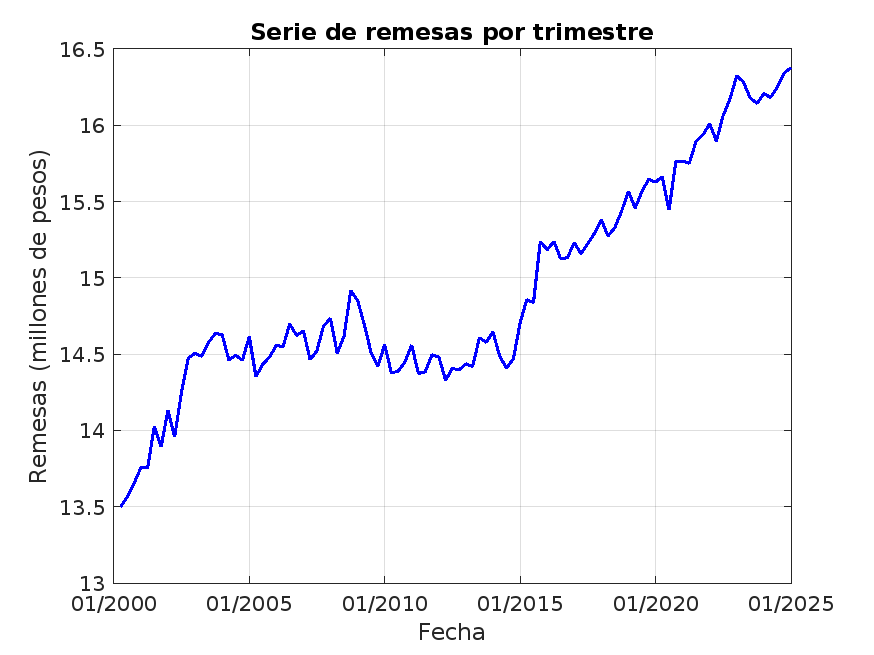
\includegraphics[width=0.5\linewidth]{docs/ln_remesastripesos.png}
    \caption{Serie de trimesas en millones de pesos colombianos}
    \label{fig:enter-label}
\end{figure}


\end{tcolorbox} 

    \item {Discuta, a la luz de la teor\'ia econ\'omica y financiera, cu\'ales de los componentes son relevantes para incluir en su modelo.}
        \begin{tcolorbox}[title=Soluci\'on 3.b]
            Es relevante incluir en el modelo para pronosticar las remesas de los trabajadores, la tendencia, la estacionalidad, los ciclos y las dinámicas de varianza. Esto debido a que la primera permite analizar los cambios positivos o negativos a través del tiempo (entre el año 2000 y 2024) del valor de las remesas así que esta nos permite observar el crecimiento de largo plazo. A su vez, la segunda nos permite identificar patrones regulares en ciertos periodos de tiempo, en este caso, si hay un incremento o una disminución de las remesas en un trimestre específico cada año. Por otra parte, es importante incluir los ciclos porque estos muestran las variaciones recurrentes que no son estacionales. Finalmente, las dinámicas de varianza también deben ser incluidas dado que no tenemos certeza sobre la homocedasticidad de la varianza, por lo que hacer uso de ellas en caso de un ruido blanco débil es clave para realizar una estimación más precisa de las remesas. 
           
                
        \end{tcolorbox}
    \item {Pruebe si es necesario incluir los componentes de tendencia y estacionalidad. De ser necesario, est\'imelos y presente sus resultados (puede probar varios modelos, pero debe continuar el desarrollo del taller con uno solo). Justifique con estad\'isticas y criterios de informaci\'on el modelo estimado.}
        
        
        \begin{tcolorbox}[title=Soluci\'on 3.c]

        \begin{figure}[H]
            \centering
            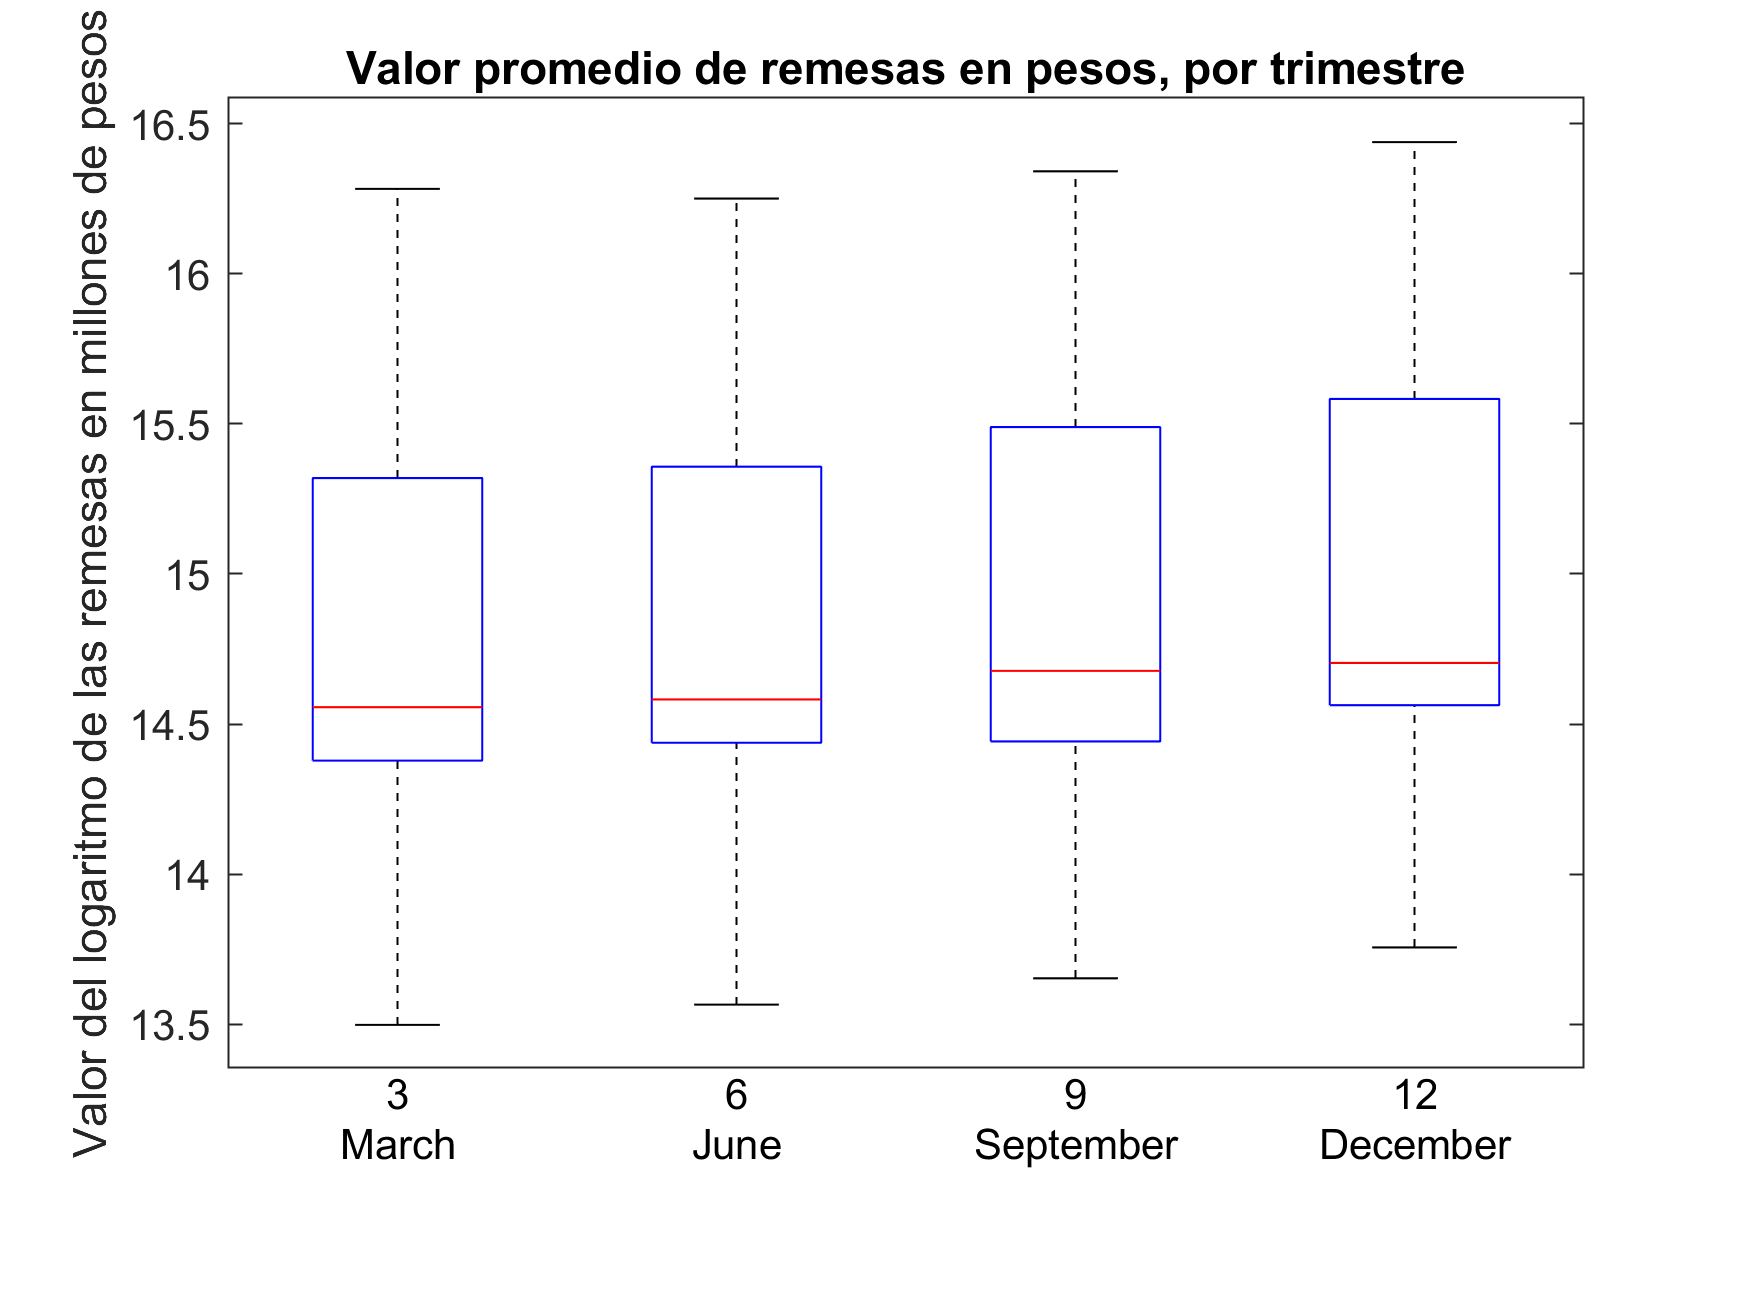
\includegraphics[width=0.5\linewidth]{docs/Remesas_Boxplot.png}
            \caption{Valor promedio de las remesas en pesos por trimestre}
            \label{fig:enter-label}
        \end{figure}
        
        \begin{figure}[H]
            \centering
            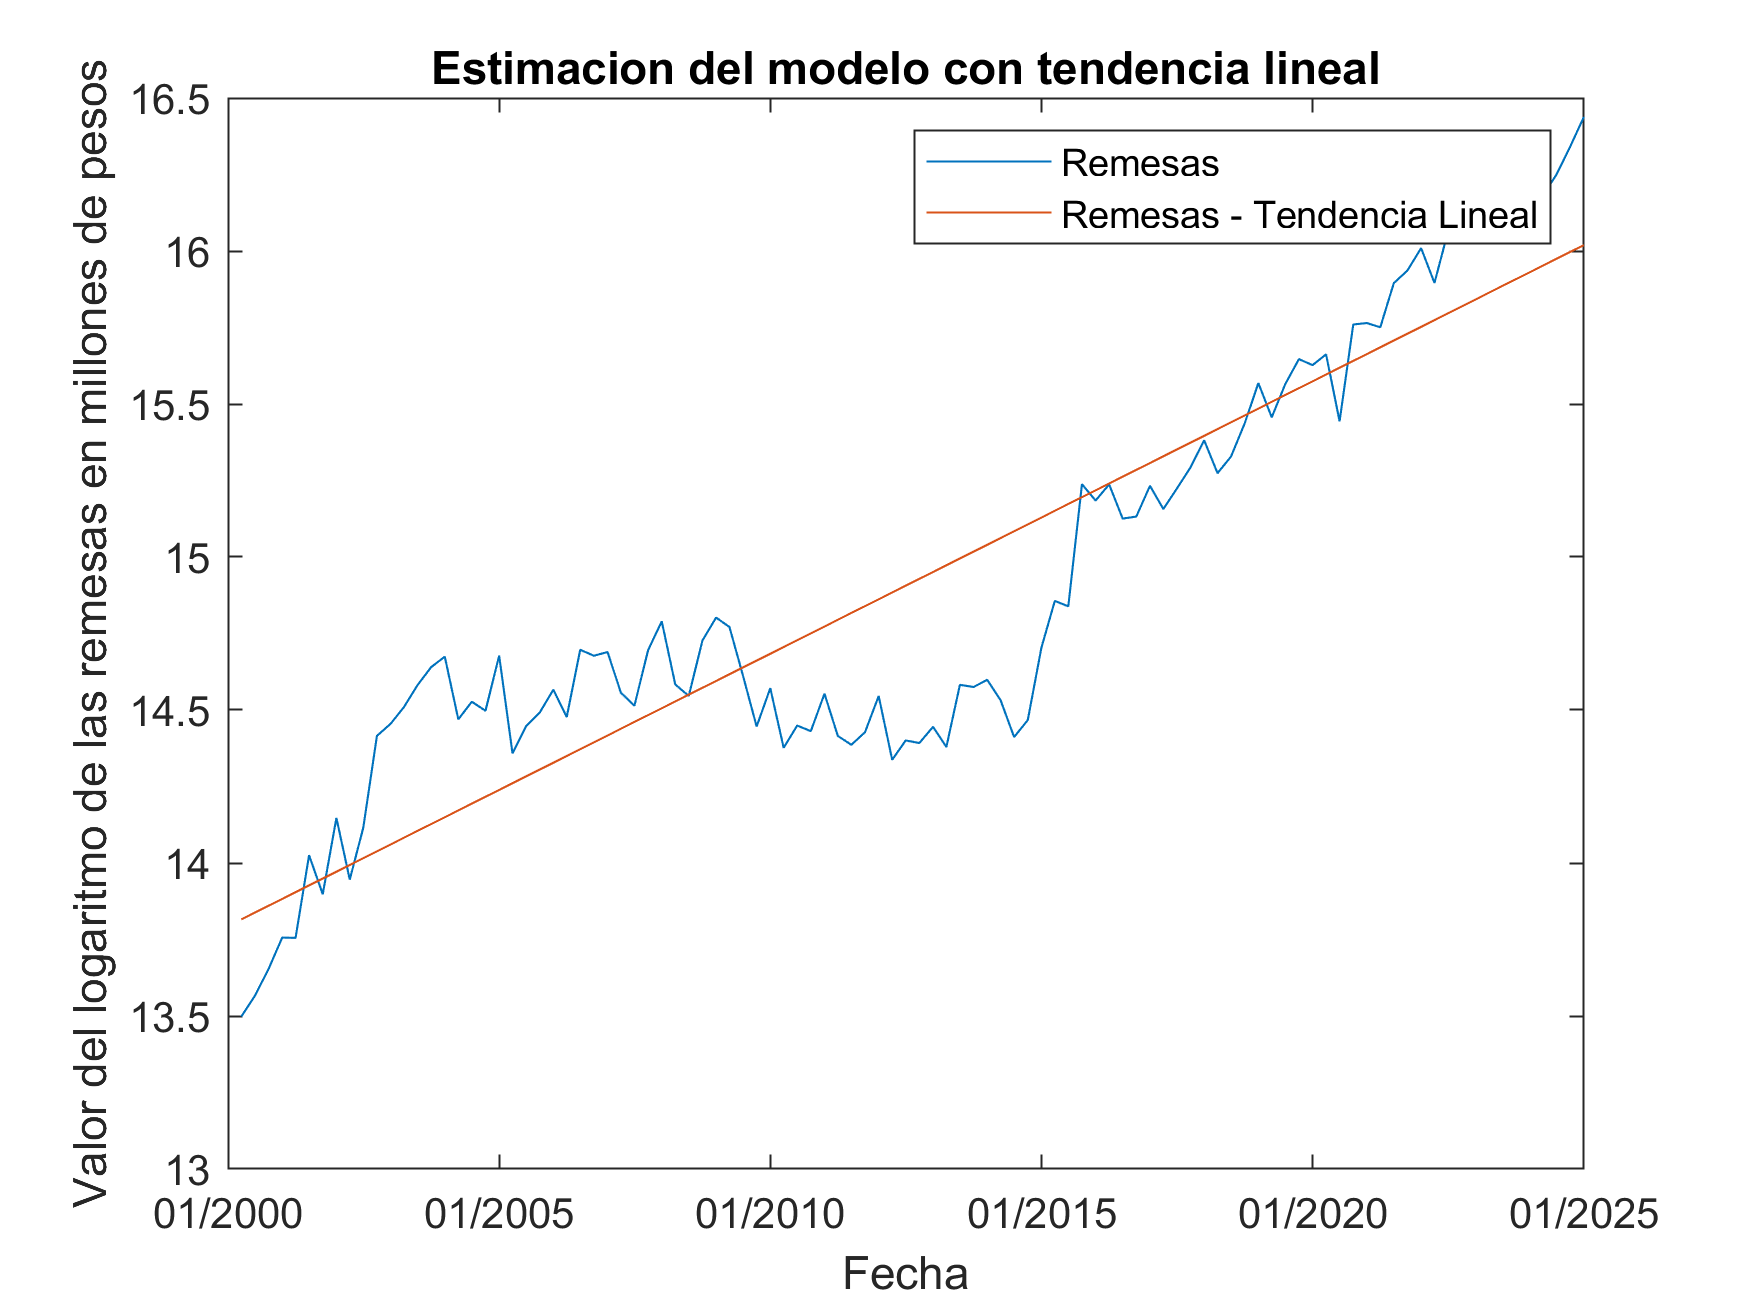
\includegraphics[width=0.5\linewidth]{docs/Remesas_tendencia_lineal.png}
            \caption{Estimación del modelo con tendencia lineal}
            \label{fig:enter-label}
        \end{figure}
            \begin{figure}[H]
                \centering
                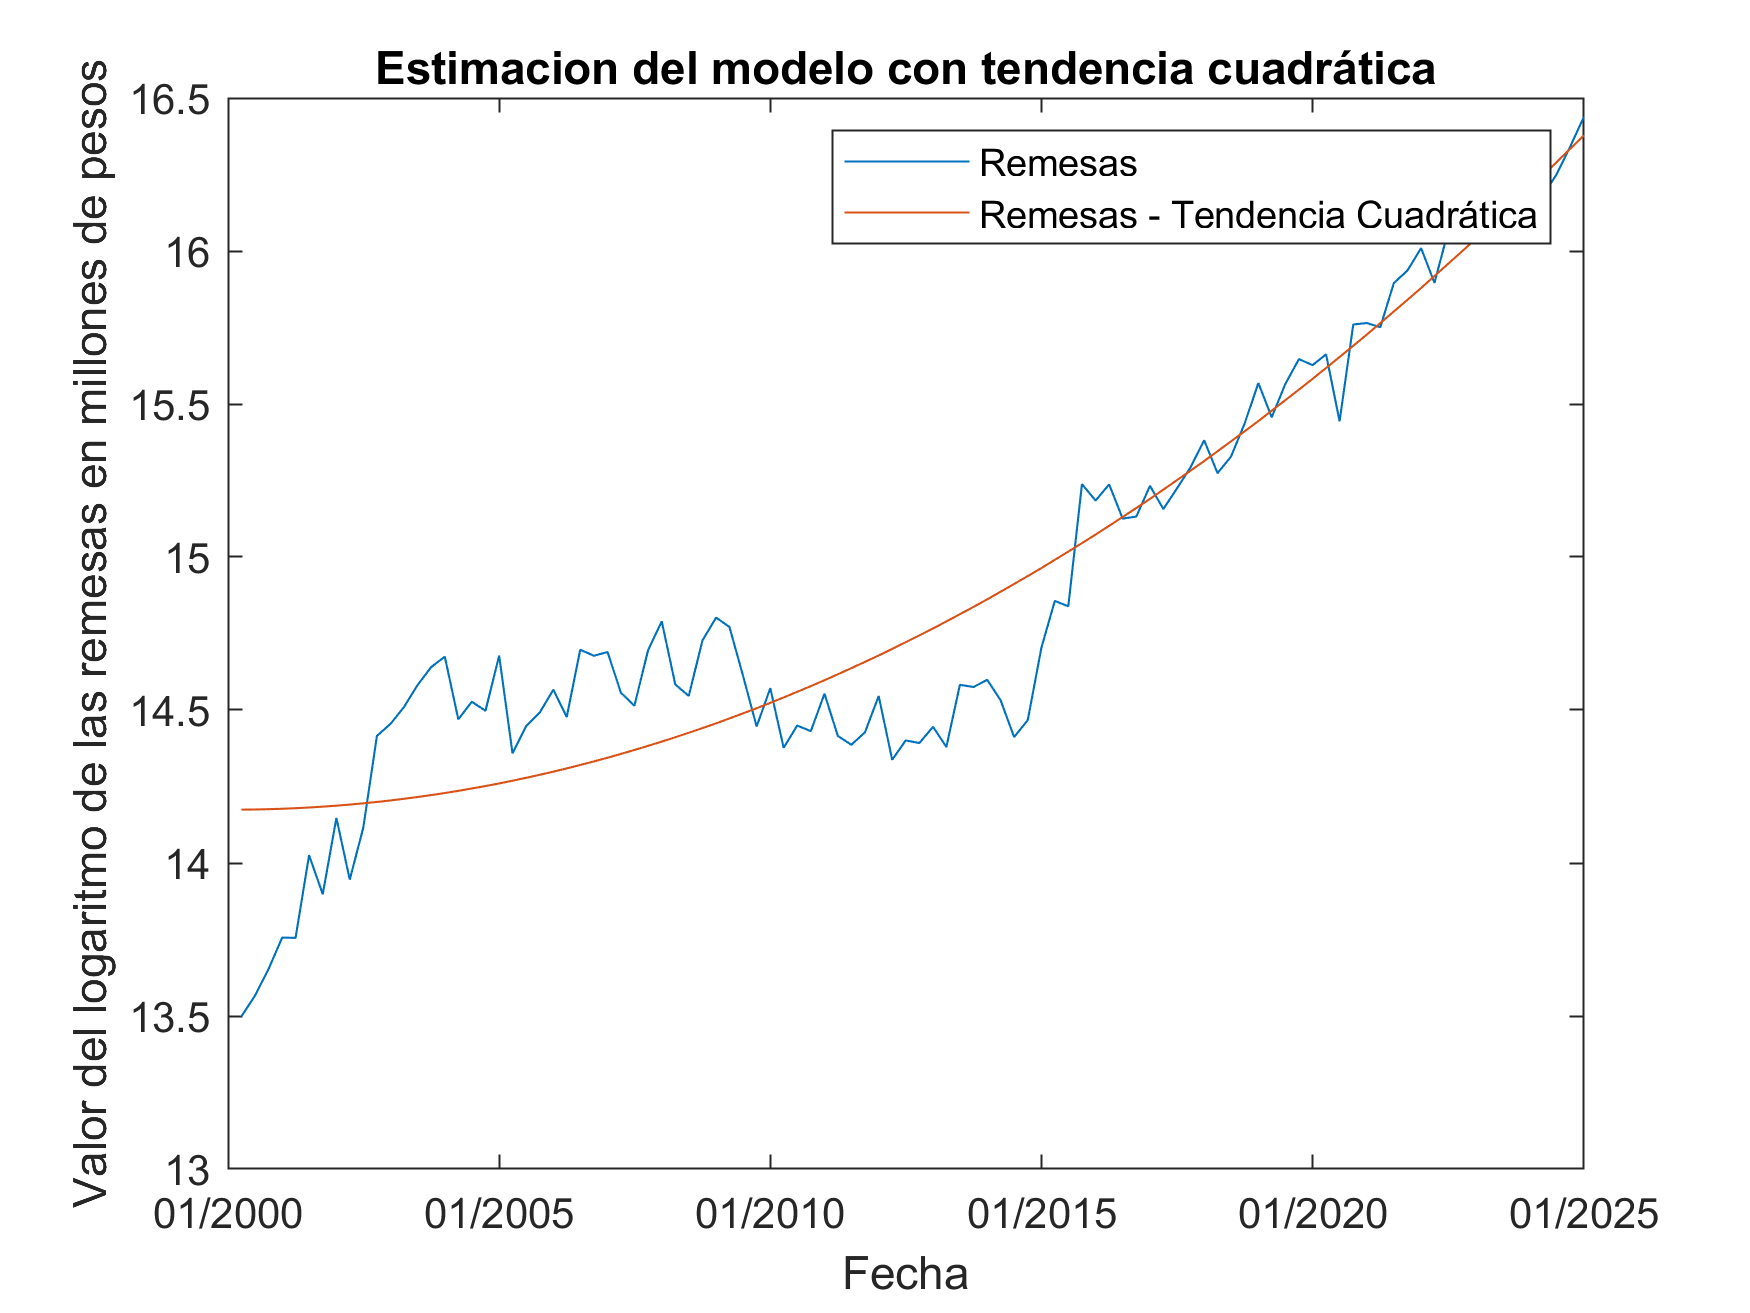
\includegraphics[width=0.5\linewidth]{docs/Remesas_tendencia_cuadratica.png}
                \caption{Estimación del modelo con tendencia cuadrática}
                \label{fig:enter-label}
            \end{figure}


       \begin{figure}[H]
            \centering
            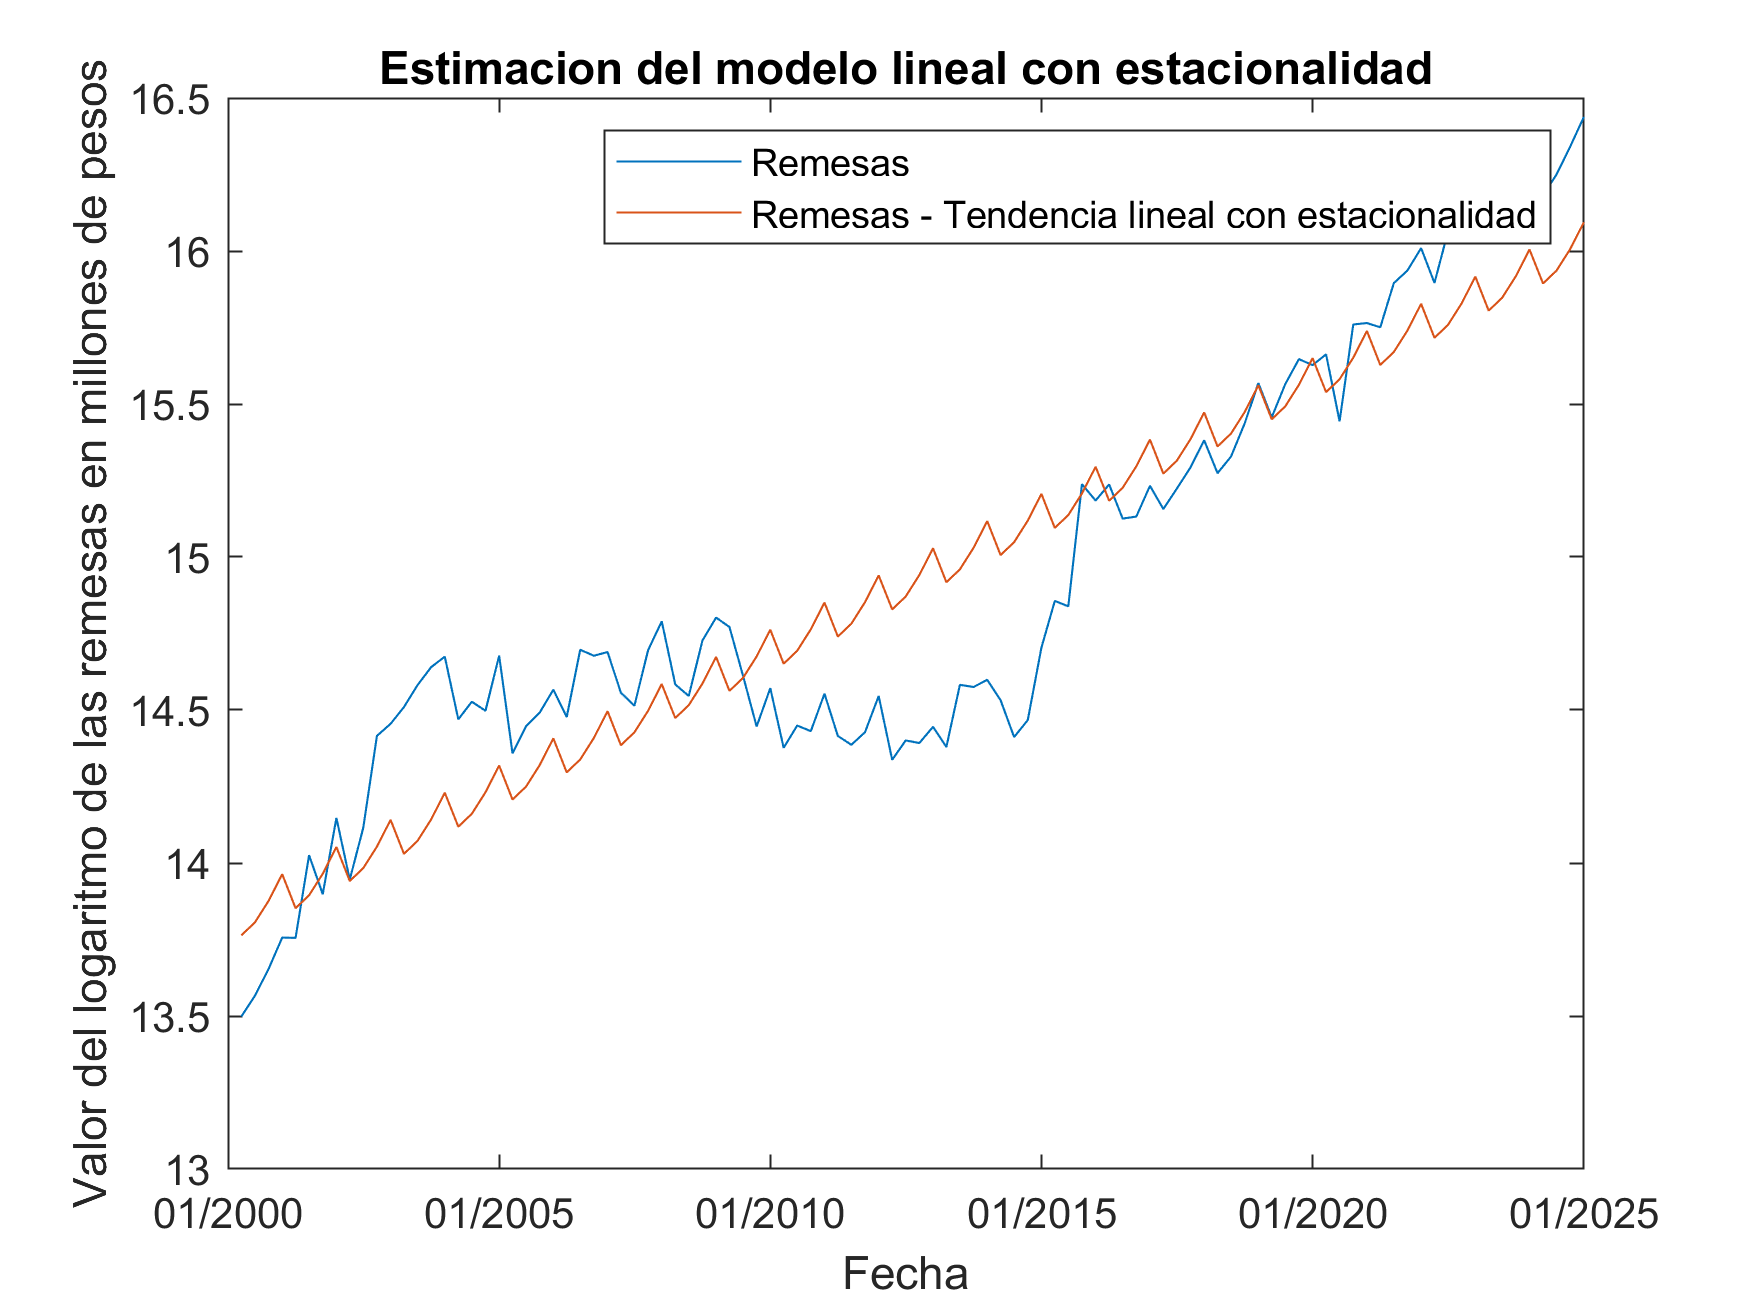
\includegraphics[width=0.5\linewidth]{docs/Remesas_estacionalidad.png}
            \caption{Estimación del modelo con tendencia lineal y con estacionalidad}
            \label{fig:enter-label}
        \end{figure}
        
        \begin{figure}[H]
            \centering
            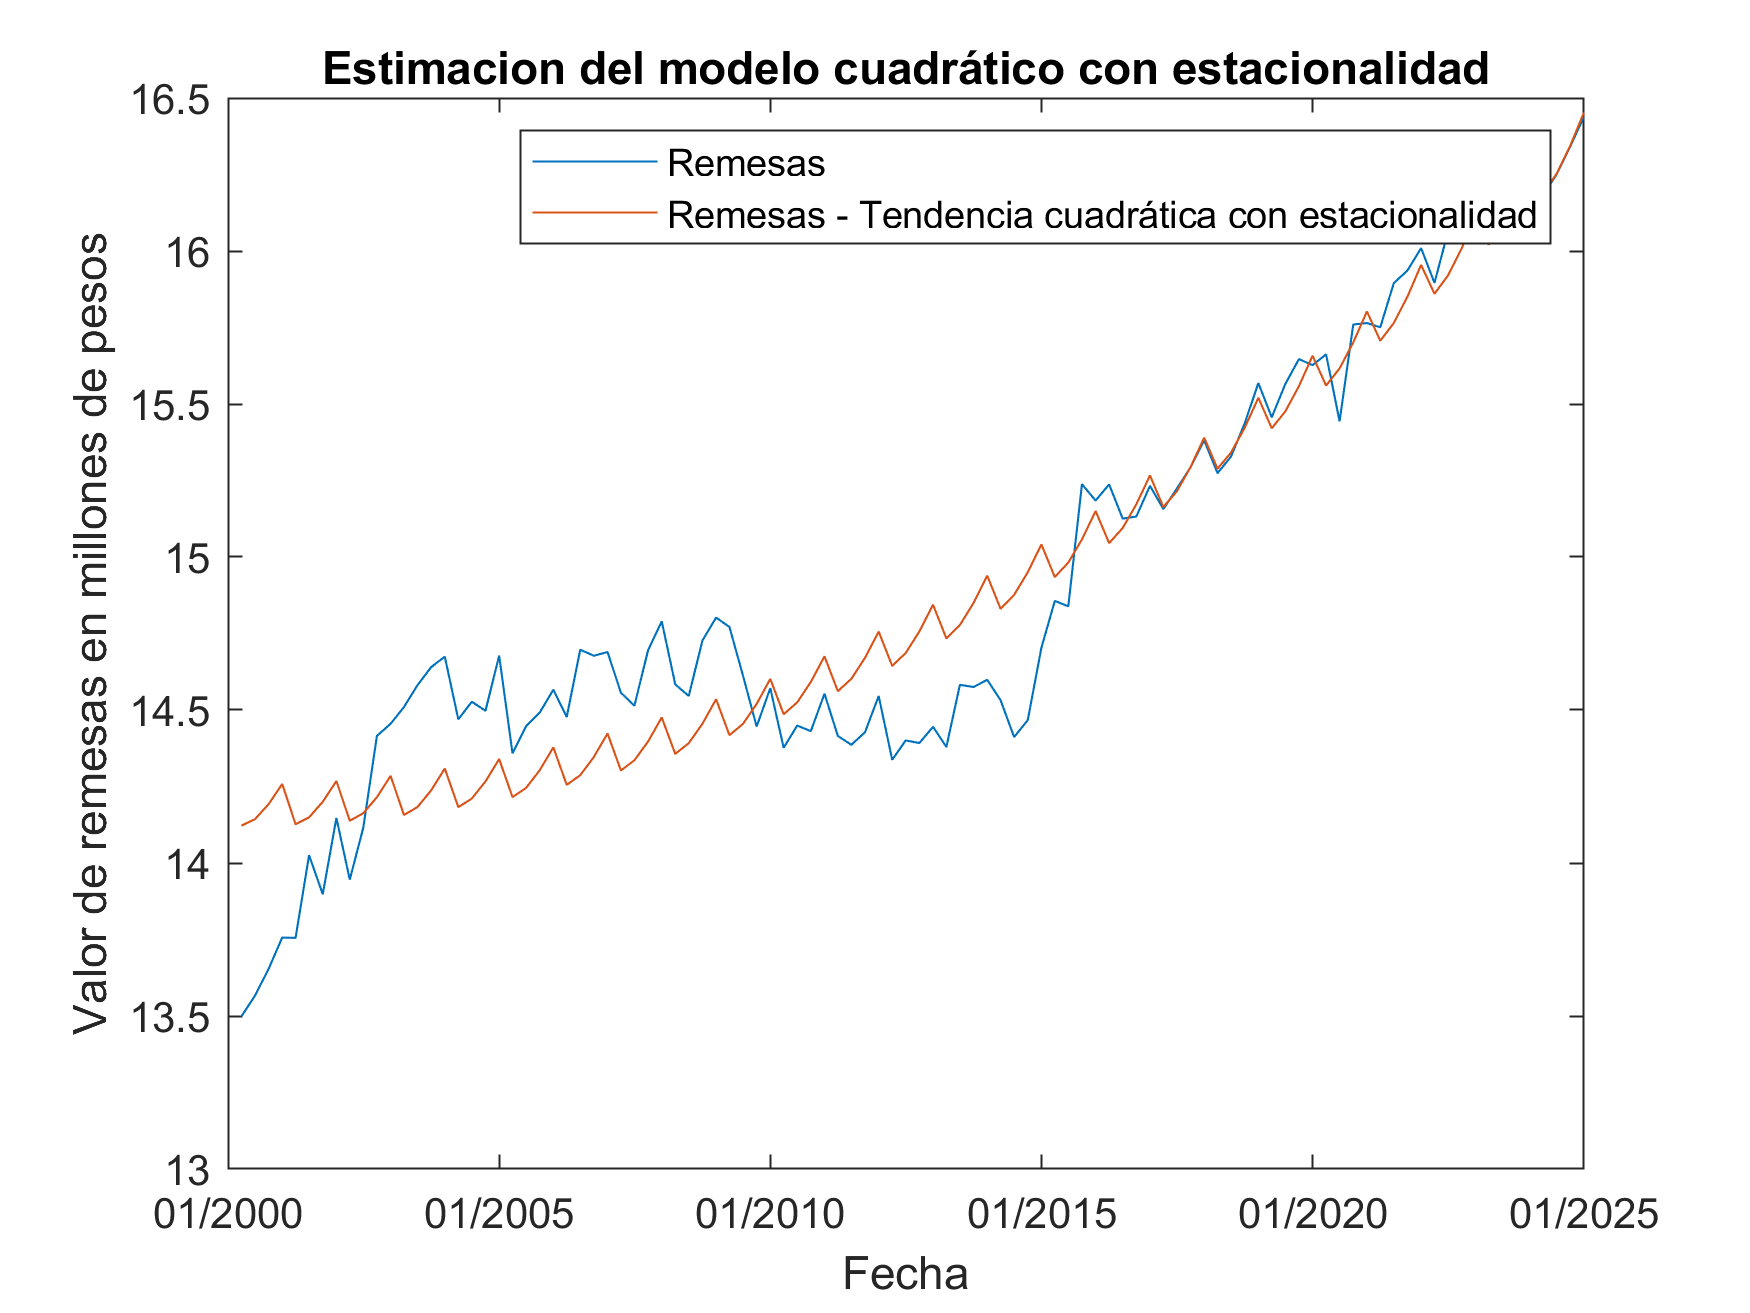
\includegraphics[width=0.5\linewidth]{docs/Remesas_cuadratico_estacionalidad.png}
            \caption{Estimación del modelo con tendencia cuadrática y estacionalidad}
            \label{fig:enter-label}
        \end{figure}


\begin{table}[H]
\centering
\scriptsize
\begin{tabular}{|l|l|l|l|}
\hline
\textbf{Modelo} & \textbf{Intercepto} & \textbf{Tiempo} & \textbf{Tiempo$^2$} \\
\hline
Beta lineal & 13.791\textsuperscript{***} & 0.022\textsuperscript{***} & --- \\
P-valor lineal & 1.82E$^{-135}$ & 8.61E$^{-39}$ & --- \\
\hline
Beta cuadrático & 14.176\textsuperscript{***} & -0.00036 & 0.00022\textsuperscript{***} \\
P-valor cuadrático & 1.10E$^{-125}$ & 0.9169 & 1.34E$^{-9}$ \\
\hline
\end{tabular}
\caption{Comparación de coeficientes y significancia entre modelos lineal y cuadrático. Notación: \textsuperscript{***} p$<$0.01, \textsuperscript{**} p$<$0.05, \textsuperscript{*} p$<$0.1}
\end{table}

\begin{table}[H]
\centering
\scriptsize
\begin{tabular}{lccccc}
\toprule
\textbf{Modelo} & \textbf{R\textsuperscript{2}} & \textbf{R\textsuperscript{2}Ajustado} & \textbf{MSE} & \textbf{AIC} & \textbf{BIC} \\
\midrule
Tendencia Lineal & 0.82388 & 0.82208 & 0.090044 & 45.021 & 50.232 \\
Tendencia Cuadrática & 0.87843 & 0.87592 & 0.062795 & 9.9543 & 17.77 \\
Lineal + Estacional & 0.82913 & 0.82193 & 0.090117 & 47.993 & 61.019 \\
Cuadrático + Estacional & 0.88367 & 0.87748 & 0.062005 & 11.546 & 27.177 \\
\bottomrule
\end{tabular}
\caption{Comparación de modelos según R\textsuperscript{2}, R\textsuperscript{2} Ajustado, MSE, AIC y BIC}
\end{table}
        
Con el objetivo de probar si es necesario incluir los componentes de tendencia y estacionalidad, primero, se creó un gráfico de cajas y bigotes para observar si el valor promedio del logaritmos las remesas era diferente según el trimestre del año. Se observa que este valor es mayor para el 3 y el 4 trimestre del año, lo que podría deberse a eventos como navidad y fin de año, donde las familias tienden a enviarse regalos, tal vez en forma de remesas. Esto podría indicar que un componente de estacionalidad podría ser incluido para pronosticar exitosamente la serie. 

\bigskip Luego, se realizó una comparación entre los coeficientes obtenidos de estimar un modelo lineal y uno cuadrático. Se llegó a la conclusión que es necesario incluir una tendencia de tipo cuadrática por varias razones. En primer lugar, al analizar al gráficas, la tendencia cuadrática presenta una forma similar a la serie de remesas y se acomoda mejor que la tendencia lineal, especialmente para los últimos valores. Por otra parte, aunque el p-valor en el modelo lineal es estadísticamente significativo, lo que sugeriría una tendencia creciente y constante a lo largo del tiempo, en el modelo cuadrático la variable de tiempo al cuadrado es estadisticamente significativa. Esto indicaría que incluir un modelo con curvatura cuadrática podría llevar a una mayor precisión en la estimación del modelo. Debido a que en ambos modelos el p-valor de los coeficientes es significativo, se recurrió a los criterios de R-cuadrado, R cuadrado ajustado, MSE y Akaike y de Shwartz, con los cuales se escogió como mejor modelo el modelo con tendencia cuadrática y estacionalidad, debido a que presenta menores valores en ambas pruebas en comparación con el modelo lineal con estacionalidad. Decidimos mantener el componente de estacionalidad, teniendo en cuenta los resultados de la gráfica de cajas y bigotes. 

        \end{tcolorbox}
    \item {Construya y grafique la serie desestacionalizada y sin tendencia.}
        \begin{tcolorbox}[title=Soluci\'on 3.d]
            \begin{figure}[H]
                \centering
                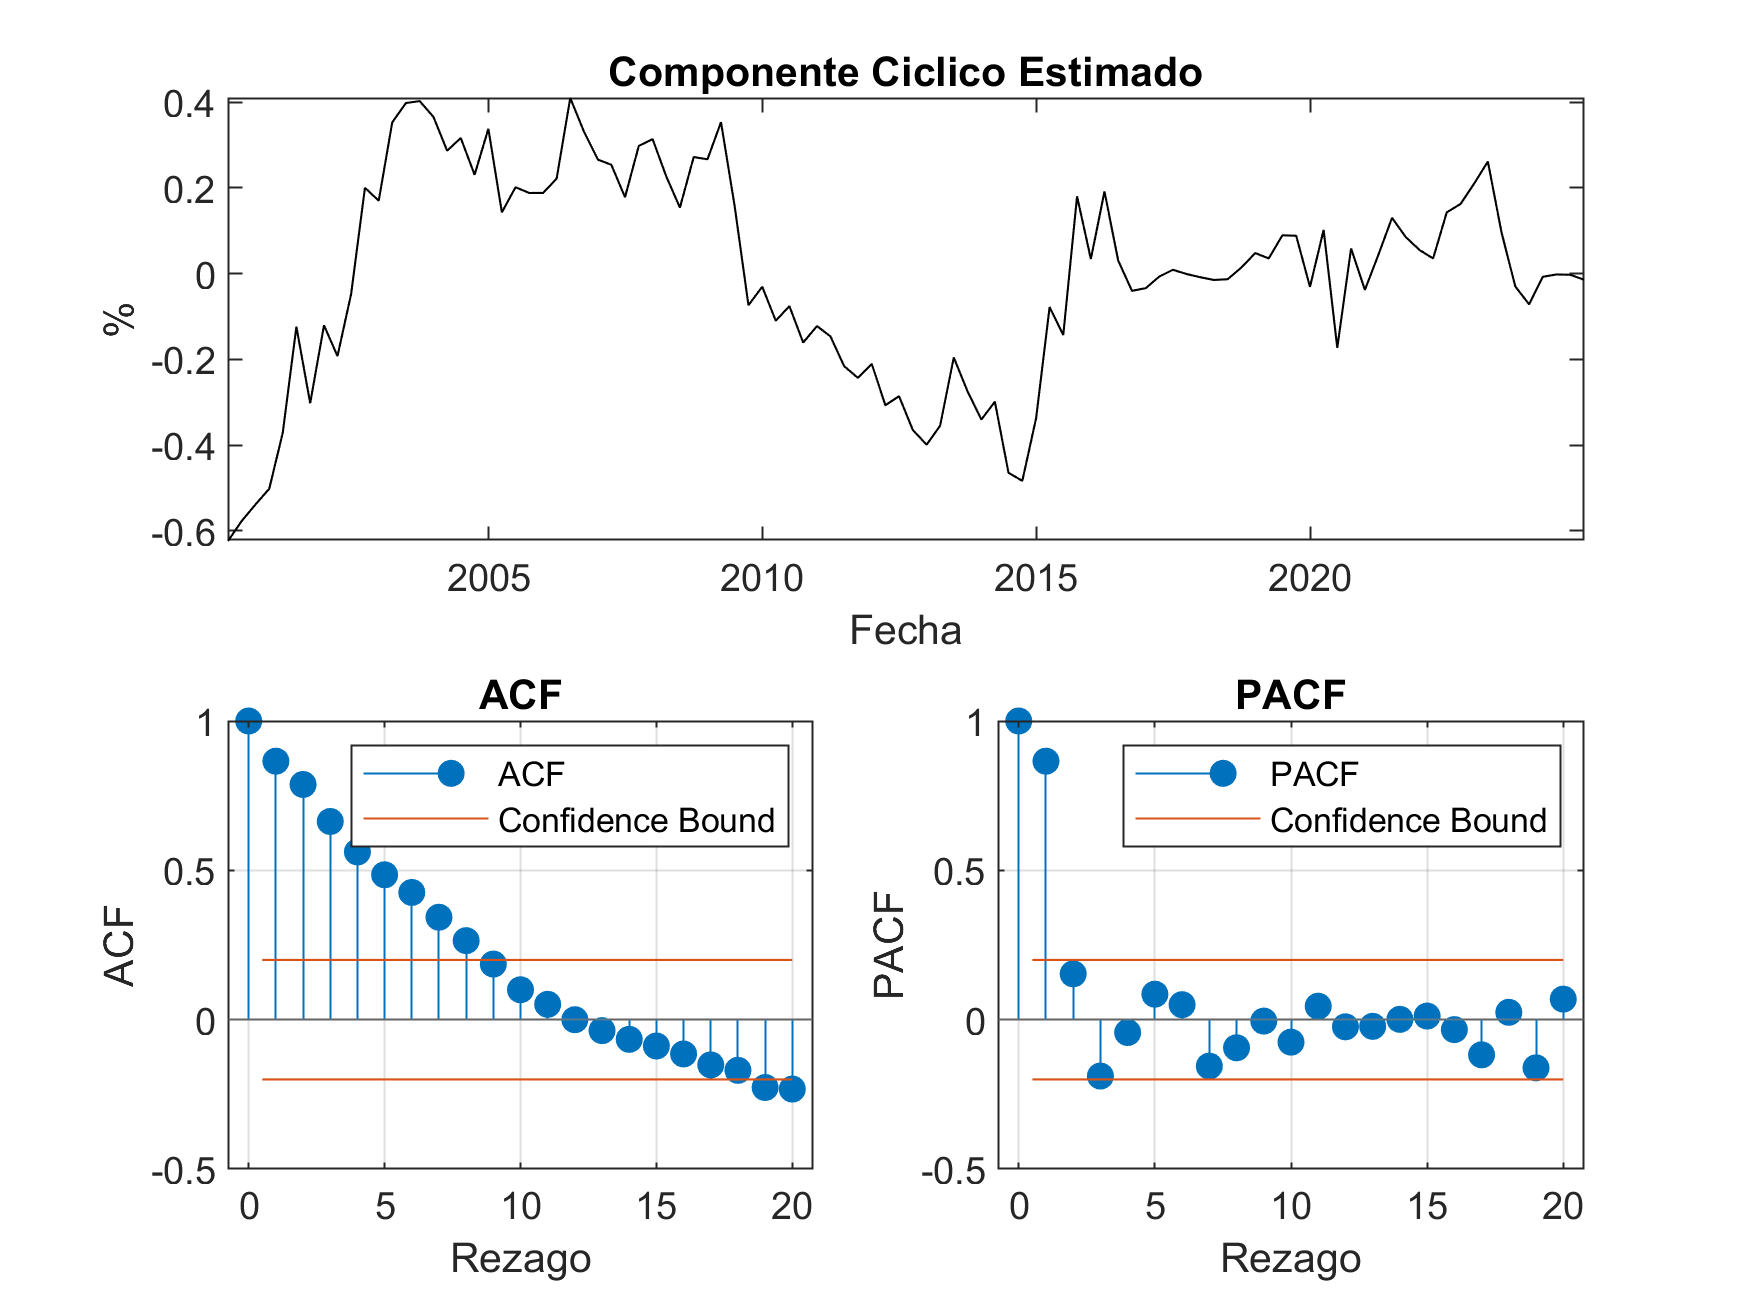
\includegraphics[width=0.5\linewidth]{docs/Serie_desestacionalizada.png}
                \caption{Componente cíclico estimado}
                \label{fig:enter-label}
            \end{figure}
            
             En la figura 16, se observa la serie del logaritmo de las remesas luego de  remover su tendencia cuadrática y su estacionalidad. La serie parece oscilar alrededor de cero y hay fluctuaciones cíclicas claras con picos y caídas. Hacia 2014, especialmente, se percibe una caída. A su vez, las gráficas de ACF y PACF muestran evidencia de autocorrelación entre los rezagos. La PACF, en específico, muestra que el primer residuo presenta autocorrelación con periodos pasados. Por esto, no se considera que la serie sea ruido blanco y se necesitan de más componentes para modelarse adecuadamente. 
        \end{tcolorbox}
    

    \item {Pruebe si es necesario incluir un componente c\'iclico. De ser necesario, estime conjuntamente el modelo con todos los componentes necesarios y presente sus resultados (puede probar varios modelos, pero debe continuar el desarrollo del taller con uno solo). Justifique con estad\'isticas y criterios de informaci\'on el modelo estimado.}
        \begin{tcolorbox}[title=Soluci\'on 3.e]
            \begin{figure}[H]
                \centering
                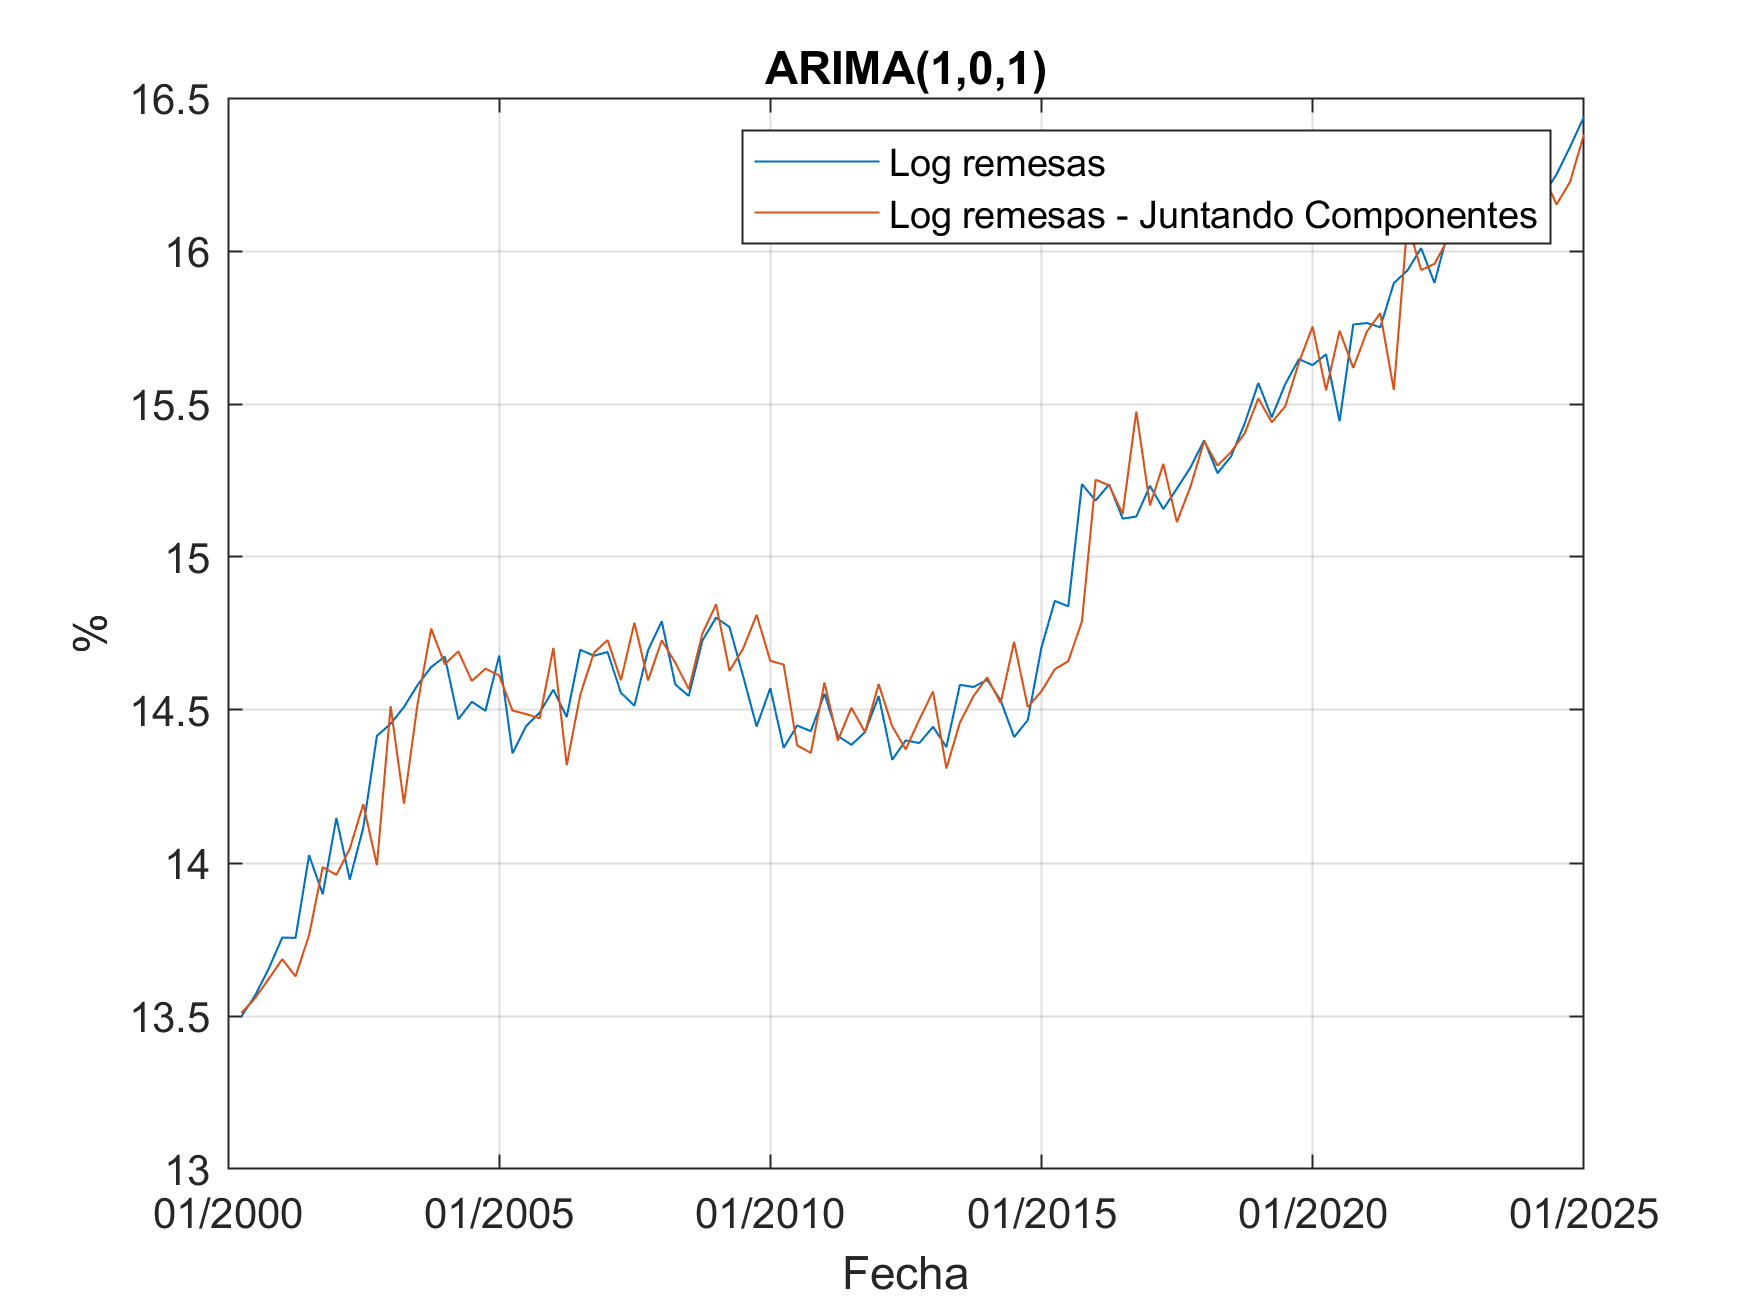
\includegraphics[width=0.5\linewidth]{docs/Arima_1_0_1.png}
                \caption{Estimación modelo ARIMA(1,0,1)}
                \label{fig:enter-label}
            \end{figure}
            \begin{figure}[H]
                \centering
                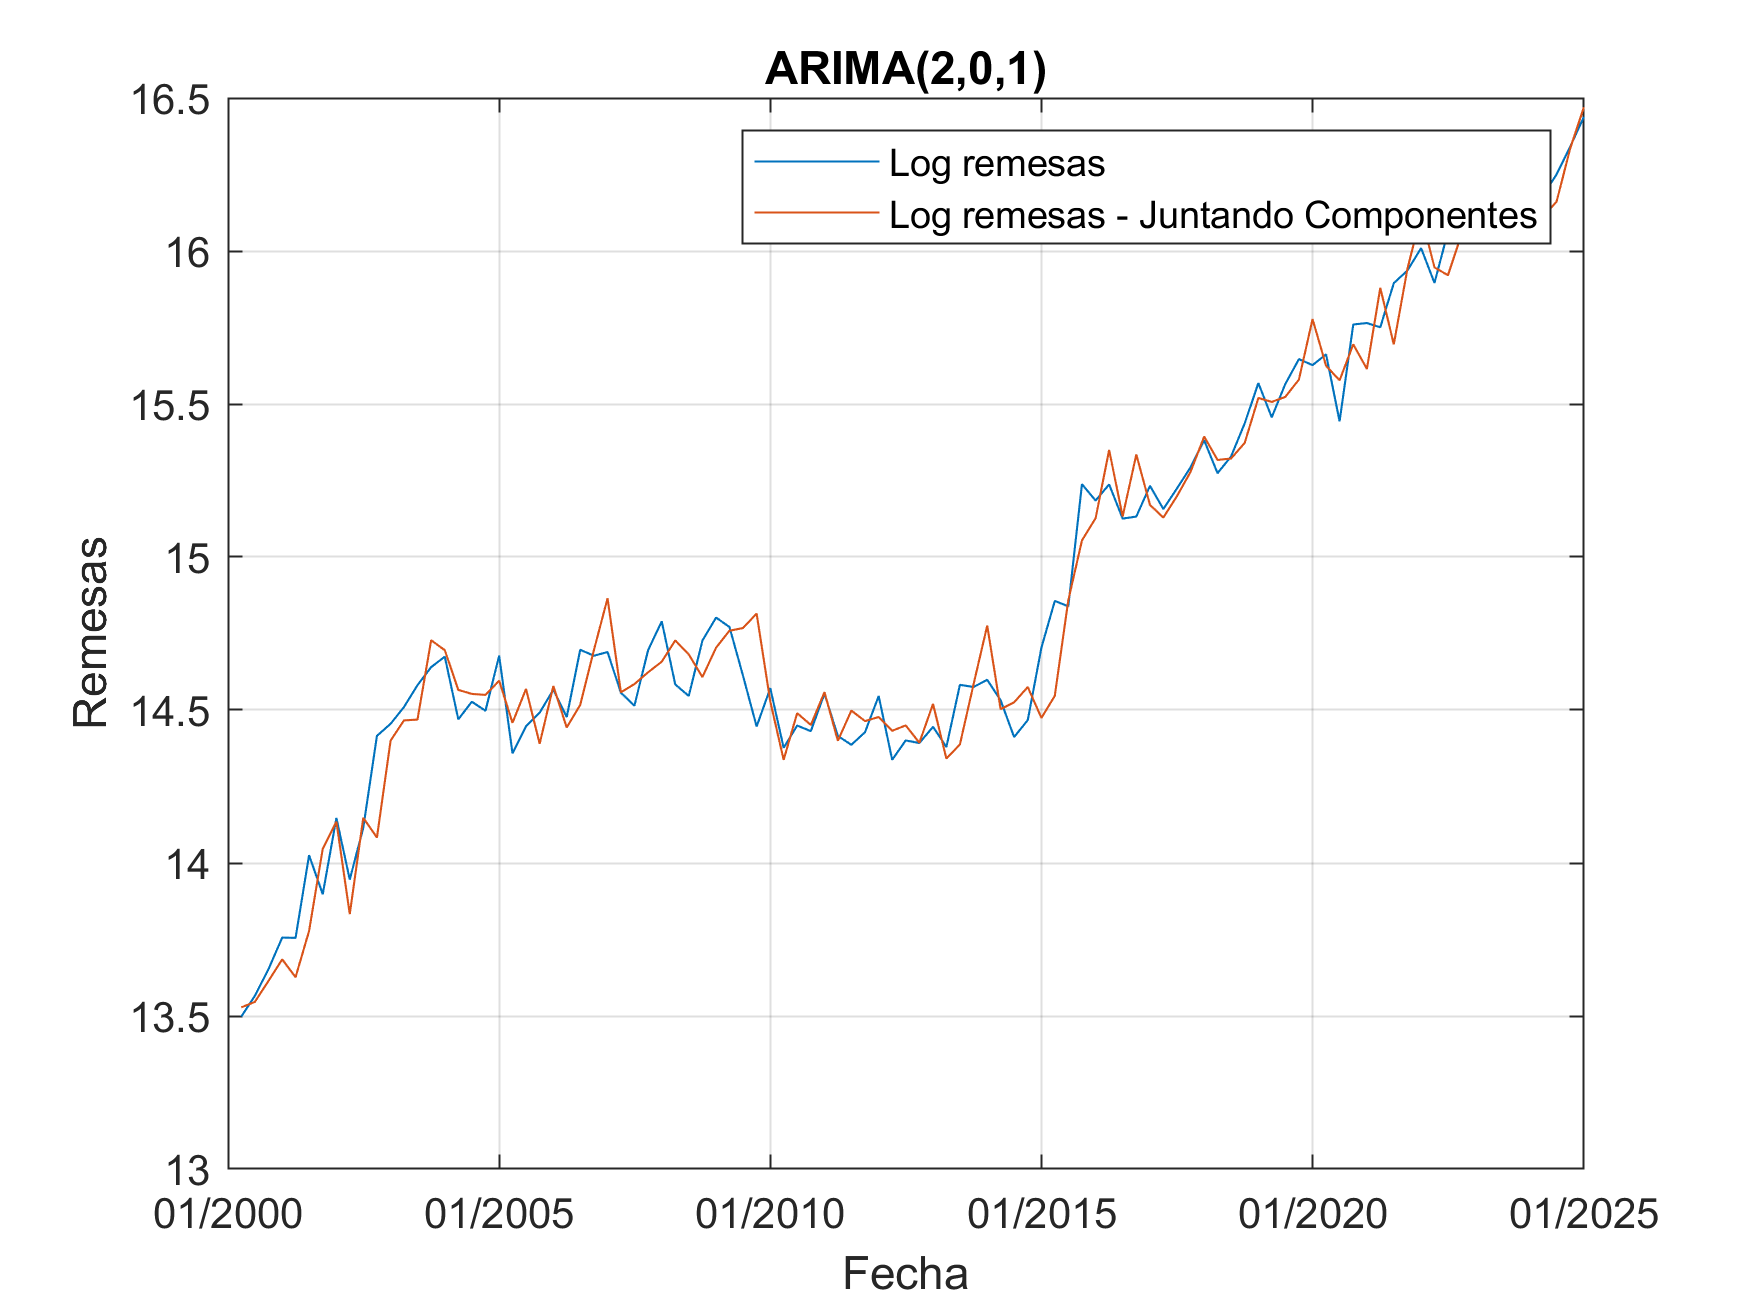
\includegraphics[width=0.5\linewidth]{docs/Arima_1_0_2.png}
                \caption{Estimación modelo ARIMA(3,0,1}
                \label{fig:enter-label}
            \end{figure}
            \begin{figure}[H]
                \centering
                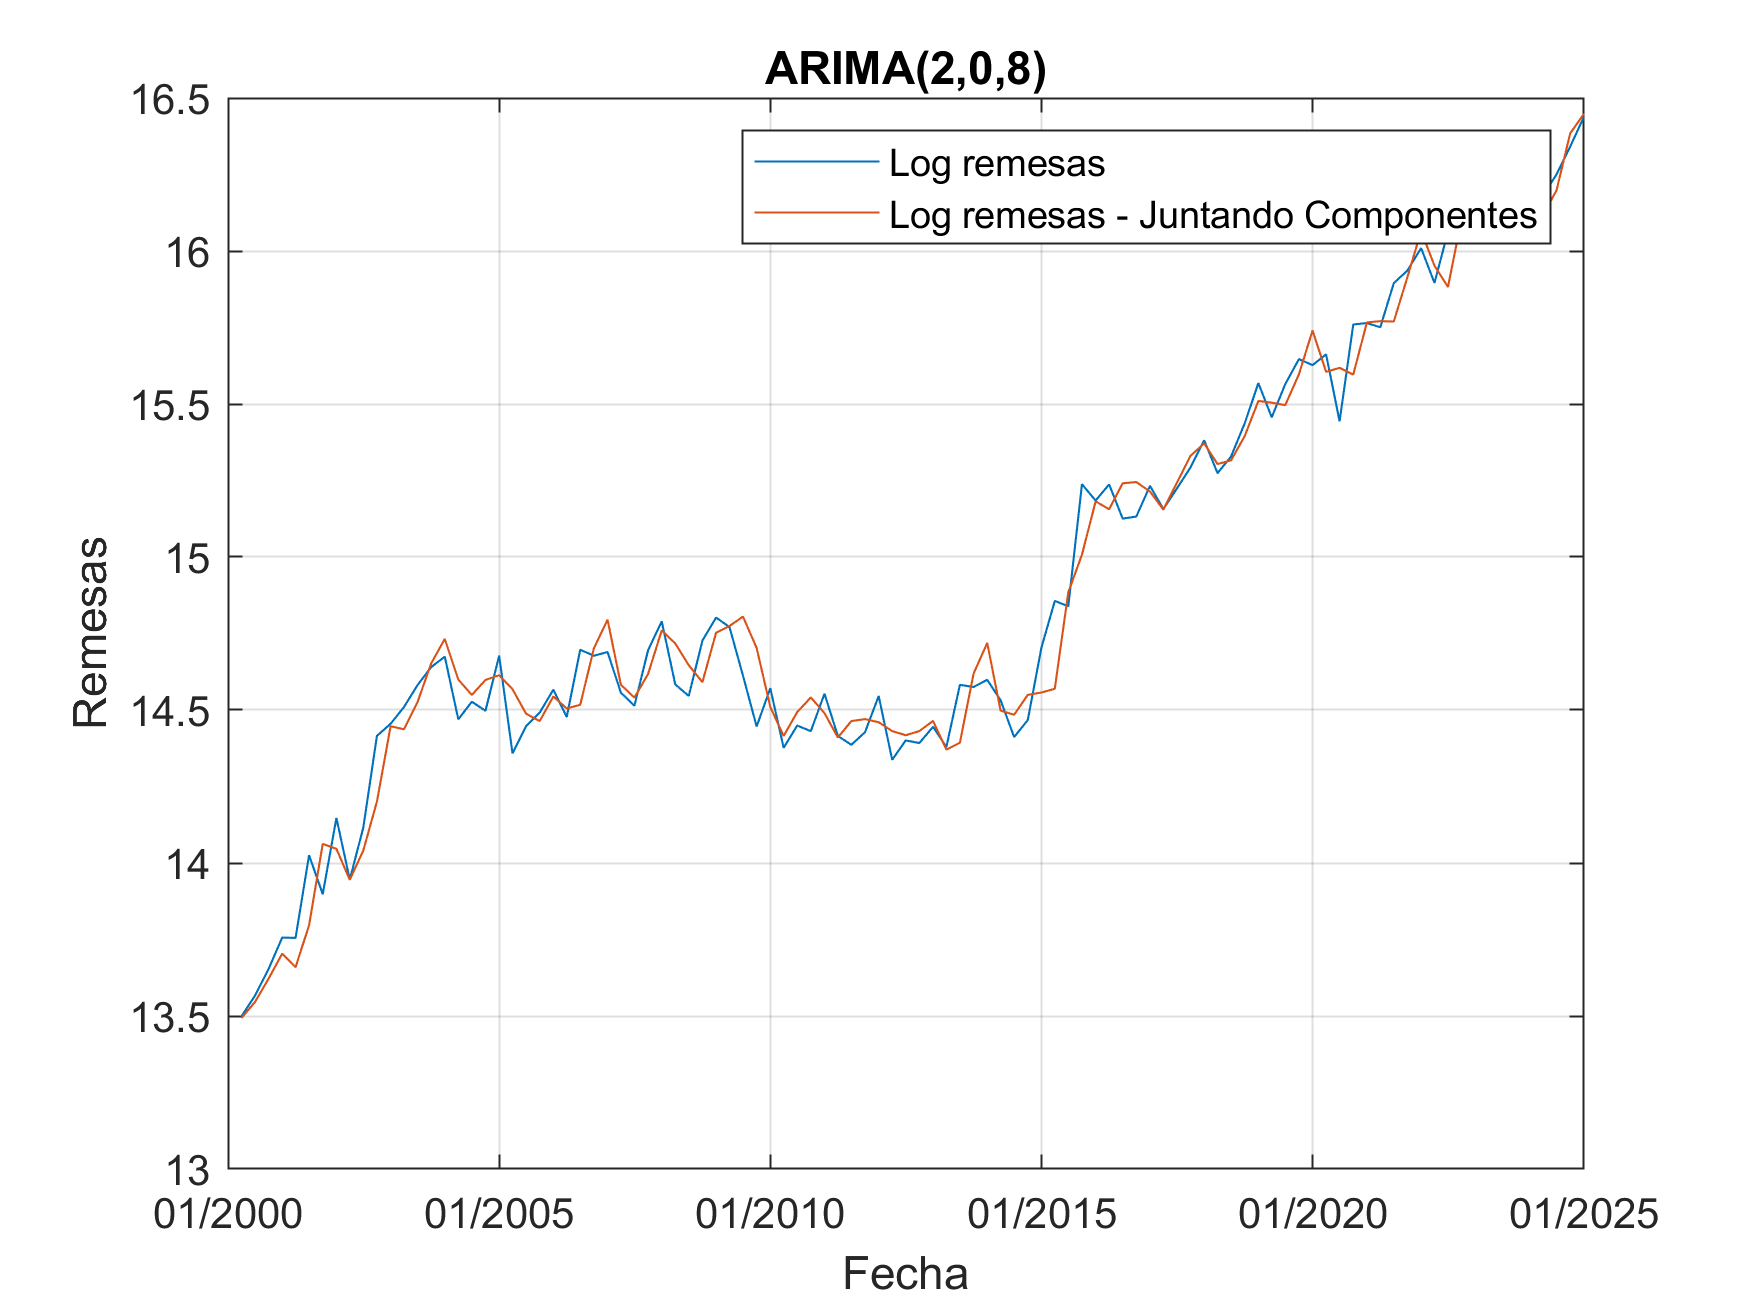
\includegraphics[width=0.5\linewidth]{docs/Arima_1_0_8.png}
                \caption{Estimación modelo ARIMA(2,0,8)}
                \label{fig:enter-label}
            \end{figure}

            \begin{figure}[H]
                \centering
                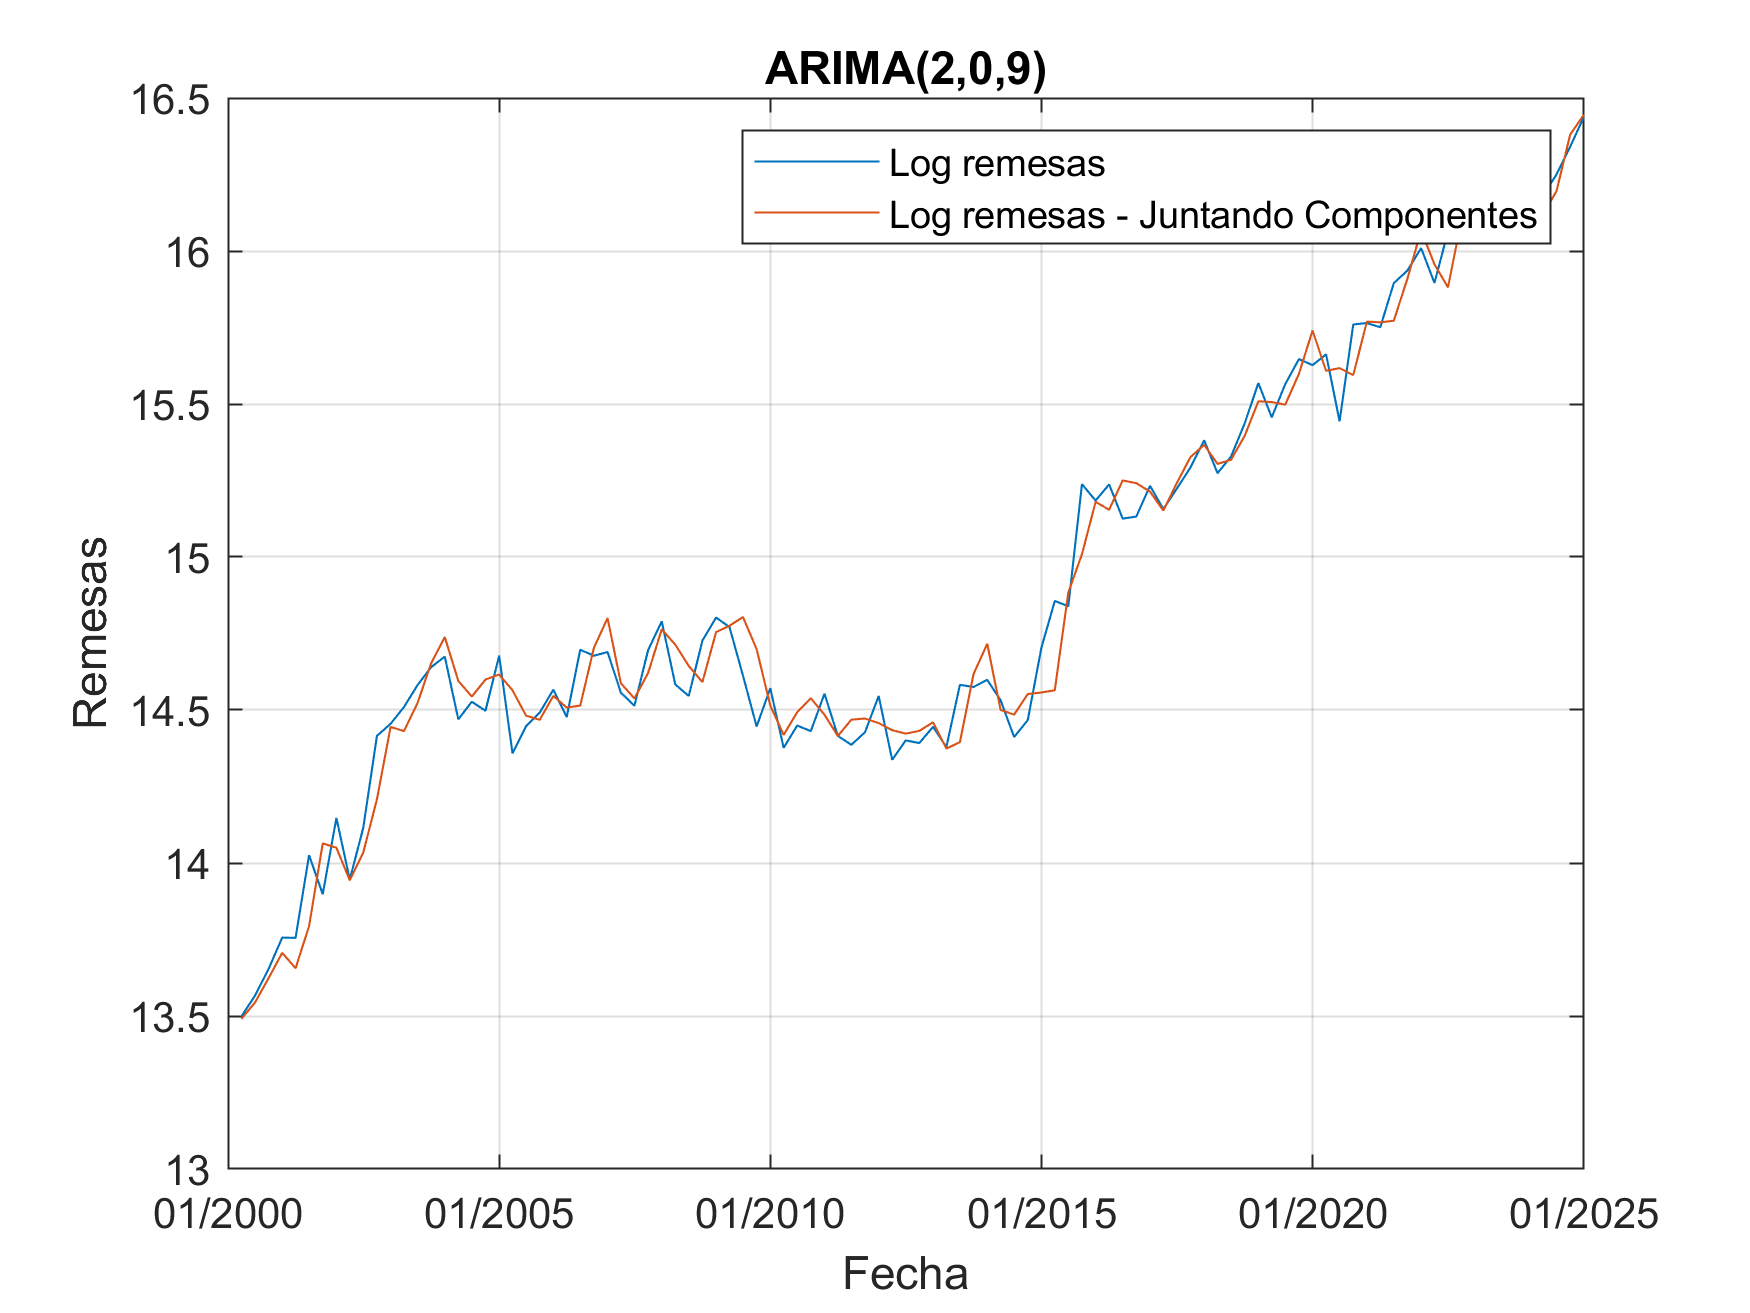
\includegraphics[width=0.5\linewidth]{docs/Arima_2_0_9.png}
                \caption{Estimación modelo ARIMA(2,0,9)}
                \label{fig:enter-label}
            \end{figure}
        \end{tcolorbox}

        
        
    \item {Construya y grafique los residuales. Justifique que se trata de ruido blanco. De ser necesario, documente las pruebas que le dan validez a sus resultados.}
        \begin{tcolorbox}[title=Soluci\'on 3.f]
            \begin{figure}[H]
                \centering
                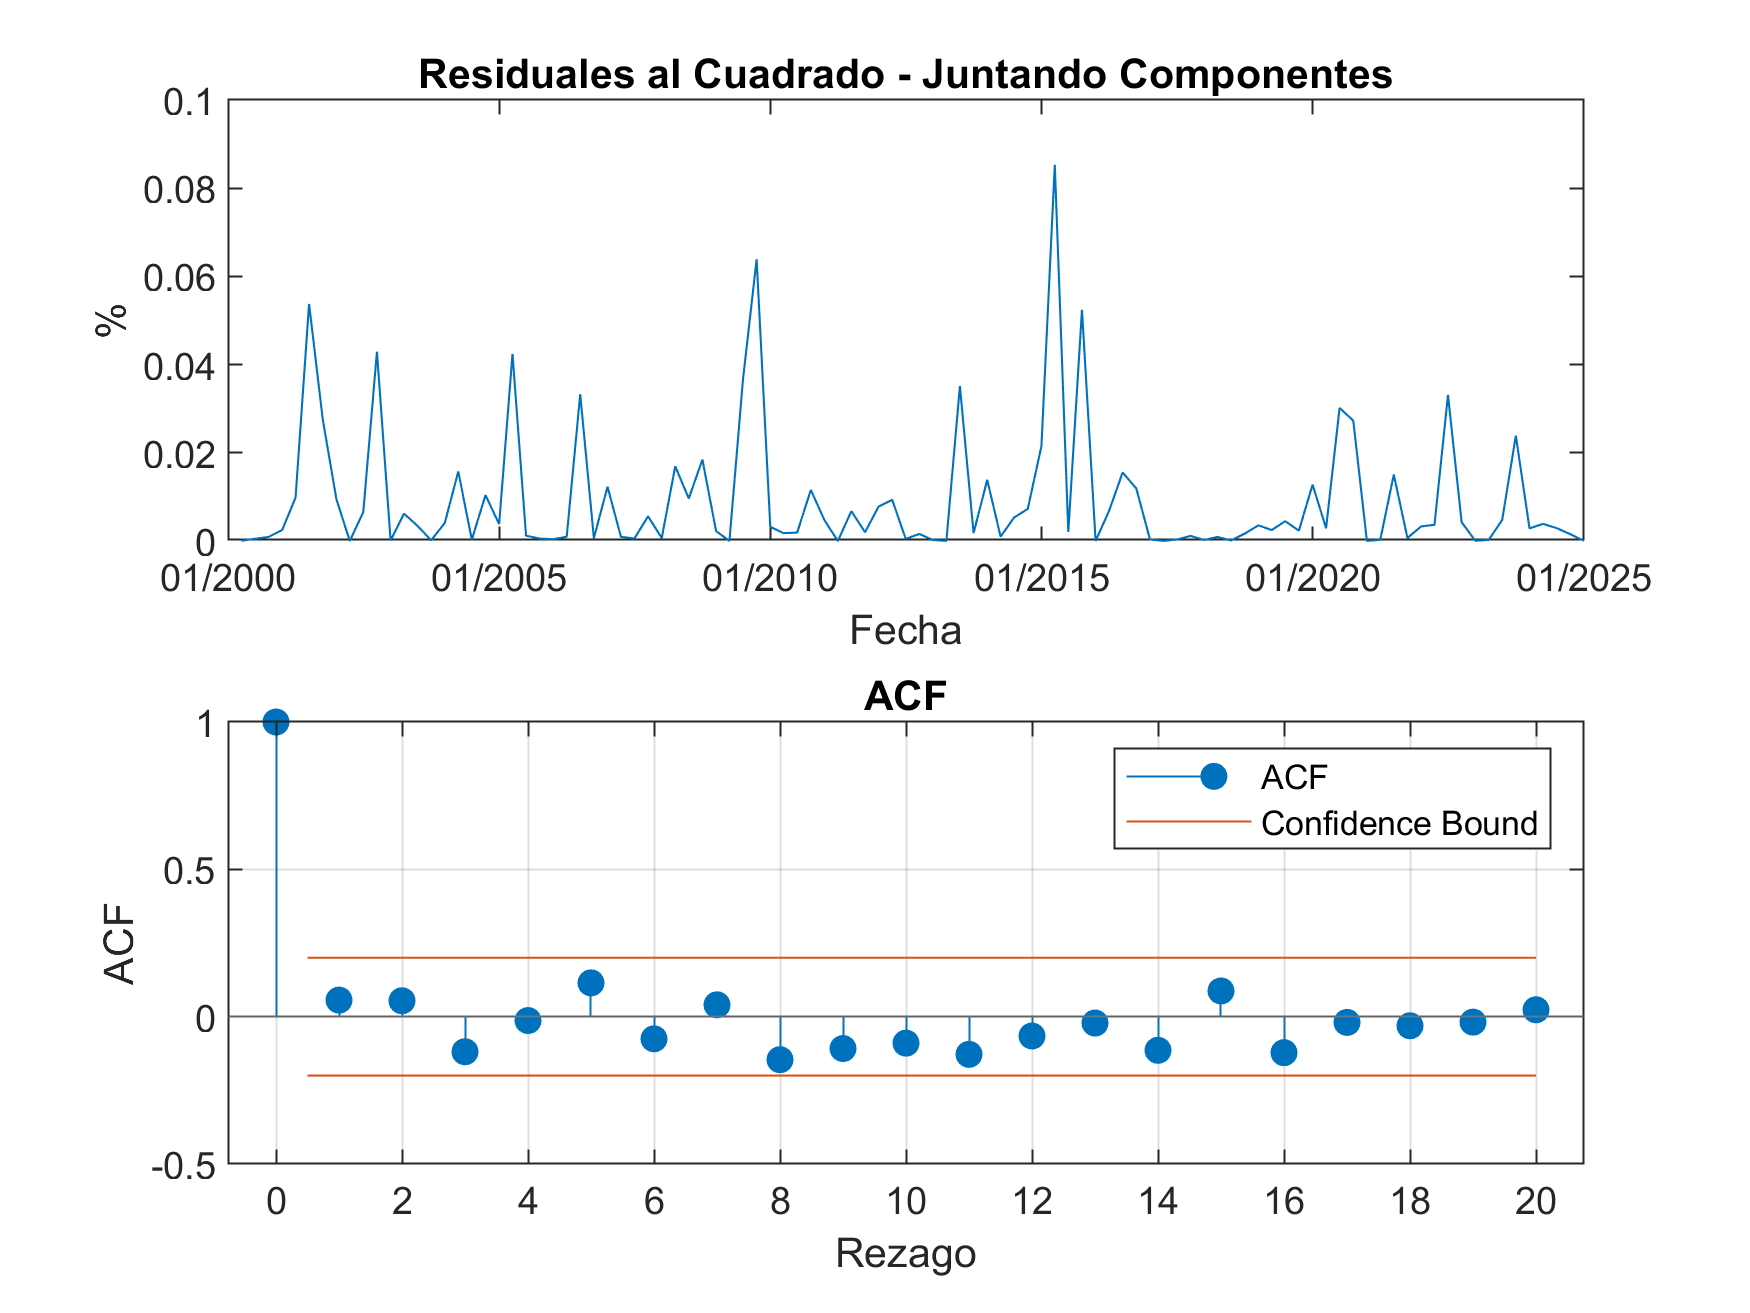
\includegraphics[width=0.5\linewidth]{docs/ARIMA_2_0_9_residuales.png}
                \caption{Residuales al cuadrado posterior a juntar componentes}
                \label{fig:enter-label}
            \end{figure}
            La estimación de los residuales al cuadrado del modelo ARIMA seleccionado posterior a unir componentes muestra que la varianza de los residuales, a pesar de presentar ciertos picos inusuales que pueden estar relacionados a choques externos, es constante. Es decir que hay homocedasticidad. Se puede concluir esto debido a que la mayoría de los residuales al cuadrado presentan valores bajos y hay ausencia de repetición cíclica. Por otra parte, la gráfica de la función de autocorrelación (ACF) de los residuales al cuadrado muestra que no hay evidencia de autocorrelación en los residuales debido a que posterior al primer rezago, los coeficientes de autocorreación caen dentro de las bandas de confianza y se mantienen dentro de estas. 
            
        \end{tcolorbox}
        
    \item {Pruebe si es necesario incluir din\'amicas de varianza condicional. De ser necesario, est\'imelas y presente sus resultados (puede probar varios modelos, pero debe continuar el desarrollo del taller con uno solo). Justifique con estad\'isticas y criterios de informaci\'on el modelo estimado.}
        \begin{tcolorbox}[title=Soluci\'on 3.g]
            
        \end{tcolorbox}
    \item {Pruebe si su modelo captura correctamente las din\'amicas de varianza. Realice y documente las pruebas necesarias.}
        \begin{tcolorbox}[title=Soluci\'on 3.h]
            
        \end{tcolorbox}
    \item {Realice el pron\'ostico puntual trimestral y simule 1.000 pron\'osticos para todo el año 2025 (i.e. pronostique los valores trimestrales de las remesas desde el primer trimestre hasta el cuarto trimestre de 2025). Sumando dichos pron\'osticos puede obtener el valor total de las remesas esperados en el año 2025. Con este valor reporte:}
    \begin{enumerate}[label=(\emph{\roman*})]
        \item {Pron\'ostico punto del total de remesas para el año 2025.}
            \begin{tcolorbox}[title=Soluci\'on 3.i.i]
            
            \end{tcolorbox}
        \item {Pron\'ostico de intervalo al 95\% de confianza del total de remesas para el año 2025.}
            \begin{tcolorbox}[title=Soluci\'on 3.i.ii]
            
            \end{tcolorbox}
        \item {Pron\'ostico de densidad del total de remesas para el año 2025. Presente sus resultados en un gr\'afico donde pueda leerse el valor de los pron\'osticos (\emph{i}) y (\emph{ii}).}
            \begin{tcolorbox}[title=Soluci\'on 3.i.iii]
            
            \end{tcolorbox}
    \end{enumerate}
\end{enumerate}

\nocite{*}

\printbibliography

\end{document}

